\documentclass[12pt, a4paper, oneside]{book}
\usepackage[hidelinks]{hyperref}
\usepackage[slovak]{babel}
\usepackage{epsfig}
\usepackage{epstopdf}
\usepackage[chapter]{algorithm}
\usepackage{algorithmic}
\usepackage{listings}
\usepackage{amsmath}
\usepackage{amssymb}
\usepackage{graphicx}
\usepackage{multirow}
\usepackage{color}
\usepackage{url}
\usepackage[utf8]{inputenc}
\usepackage[T1]{fontenc}
\usepackage{setspace}
\usepackage{tabularx}
\usepackage{textcomp}
\usepackage{caption}
\usepackage{natbib}
\usepackage{pdfpages}
\usepackage[none]{hyphenat}
\tolerance=1
\emergencystretch=\maxdimen
\hyphenpenalty=10000
\hbadness=10000

% TODO NOTES
\usepackage{todonotes}
%\usepackage[disable]{todonotes}
\usepackage{xcolor}
\usepackage[normalem]{ulem}
\usepackage{soul}

%%% TODO Notes
\newcommand{\assignment}[2][]{\todo[caption={},inline,bordercolor=green!67!yellow!75!black!50,color=green!67!yellow!25,size=\footnotesize,#1]{#2}}
\newcommand{\overview}[2][]{\todo[caption={},inline,color=blue!85!green!25,bordercolor=blue!85!green!50!black!50,size=\footnotesize,#1]{#2}}
\newcommand{\minor}[2][]{\todo[caption={},color=gray!30,bordercolor=gray,inline,size=\footnotesize,#1]{#2}}
\newcommand{\cutting}[2][]{\todo[color=yellow!30,bordercolor=yellow!50!black!50,inline,size=\footnotesize,#1]{#2}}
\newcommand{\bigassignment}[2][]{\todo[inline, caption={Big assignment},
    color=green!40, #1]{\begin{minipage}{\textwidth-4pt}#2\end{minipage}}}
\newskip\movedskip
\newcommand{\movespaceafter}[1]{%
    \movedskip=0pt%
    \ifhmode\ifdim\lastskip=0pt\else\movedskip=\lastskip\unskip\fi\fi
    #1\ifdim\movedskip=0pt\else\hskip\movedskip\fi
    \ignorespaces}
\newcommand{\reviewnote}[3][]{%
  \movespaceafter{\todo[inline,color=yellow!75!white,linecolor=yellow!85!black,#1]
      {\textsf{\bfseries Review #2:} \ignorespaces#3\par}}%
}
%\newcommand{\comment}[3][]{%
%  \movespaceafter{\todo[color=green!40,#1]
%      {\textsf{\bfseries #2:} \ignorespaces#3\par}}%
%}

\definecolor{mossgreen}{HTML}{146614}
\newcommand{\del}[1]{\color{red}\sout{#1}\color{black}\@}
\newcommand{\ins}[1]{\color{mossgreen}\uwave{#1}\color{black}\@}
\newcommand{\sug}[2]{\del{#1}\ins{#2}}

\newcommand{\UP}{$\uparrow$}
\newcommand{\DOWN}{$\downarrow$}
\newcommand{\UD}{$\updownarrow$}



\setstretch{1.5}
%\renewcommand\baselinestretch{1.5} % riadkovanie jeden a pol

% pekne pokope definujeme potrebne udaje
\newcommand\mftitle{Sémantické publikovanie spravodajských dát}
\newcommand\mftitlen{o bezpečnostných hrozbách}
\newcommand\mfthesistype{Diplomová práca}
\newcommand\mfauthor{Bc. Matej Rychtárik}
\newcommand\mfadvisor{doc. RNDr. Martin Homola, PhD.}
\newcommand\mfconsultant{Ing. Štefan Balogh, PhD.}
\newcommand\mfplacedate{Bratislava, 2021}
\newcommand\mfuniversity{UNIVERZITA KOMENSKÉHO V BRATISLAVE}
\newcommand\mffaculty{FAKULTA MATEMATIKY, FYZIKY A INFORMATIKY}
\newcommand{\sub}[1]{$_{\text{#1}}$}
\newcommand{\reference}[1]{č.~\ref{#1}}
\newcommand{\imageHeight}{150px}

\ifx\pdfoutput\undefined\relax\else\pdfinfo{ /Title (\mftitle) /Author (\mfauthor) /Creator (PDFLaTeX) } \fi

\begin{document}

\frontmatter

\thispagestyle{empty}

\noindent
\begin{minipage}{\textwidth}
\begin{center}
\textbf{\mfuniversity \\
\mffaculty}
\end{center}
\end{minipage}

\vfill
\begin{figure}[!hbt]
	\begin{center}
		
\includegraphics{images/logo_fmph}
		\label{img:logo}
	\end{center}
\end{figure}
\begin{center}
	\begin{minipage}{0.8\textwidth}
		\centerline{\textbf{\large\MakeUppercase{\mftitle}}}
		\centerline{\textbf{\large\MakeUppercase{\mftitlen}}}
		\smallskip
		\centerline{\mfthesistype}
	\end{minipage}
\end{center}
\vfill
2021 \hfill
\mfauthor
\eject 
% koniec obalu

\thispagestyle{empty}

\noindent
\begin{minipage}{\textwidth}
\begin{center}
\textbf{\mfuniversity \\
\mffaculty}
\end{center}
\end{minipage}

\vfill
\begin{figure}[!hbt]
\begin{center}

\includegraphics{images/logo_fmph_dark}
\label{img:logo_dark}
\end{center}
\end{figure}
\begin{center}
\begin{minipage}{0.8\textwidth}
\centerline{\textbf{\large\MakeUppercase{\mftitle}}}
\centerline{\textbf{\large\MakeUppercase{\mftitlen}}}
\smallskip
\centerline{\mfthesistype}
\end{minipage}
\end{center}
\vfill
\begin{tabular}{l l}
%Registration number: & 40a99bd8-3cb6-4534-9330-c7fd9b5e5ca4 \\
Študijný program: & Aplikovaná informatika\\
Študijný odbor: & 2511 Aplikovaná informatika\\
Školiace pracovisko: & Katedra aplikovanej informatiky\\
Školiteľ: & \mfadvisor \\
Konzultant: & \mfconsultant
\end{tabular}
\vfill
\noindent
\mfplacedate \hfill
\mfauthor
\eject 
% koniec titulneho listu

%\thispagestyle{empty}
%\includegraphics[width=\textwidth]{images/zadanie}
%\vfill
%\eject
% koniec zadania
\includepdf[pages={1}]{zadanie.pdf}

\thispagestyle{empty}

%\includepdf[pages=1,scale=1]{zadanie.pdf}

{~}\vspace{12cm}

\noindent
\begin{minipage}{0.25\textwidth}~\end{minipage}
\begin{minipage}{0.75\textwidth}
Čestne prehlasujem, že túto diplomovú prácu som vypracoval samostatne len s použitím uvedenej literatúry a za pomoci konzultácií u môjho školiteľa a konzultanta.
\newline \newline
\end{minipage}
\vfill
~ \hfill {\hbox to 6cm{\dotfill}} \\
\mfplacedate \hfill \mfauthor
\vfill\eject 
% koniec prehlasenia

\chapter*{Poďakovanie}\label{chap:thank_you}
Touto cestou by som sa chcel v prvom rade poďakovať môjmu školiteľovi, Martinovi Homolovi, a konzultantovi, Štefanovi Baloghovi, za ich cenné rady a usmernenia, ktoré mi veľmi pomohli pri riešení tejto diplomovej práce. 
\assignment{MH: Nezabudni podakovat sa aj Stefanovi. Inak tu tituly mozes vypustit, my dvaja si ozaj na to nepotrpime ;)}
\vfill\eject 
% koniec podakovania

\chapter*{Abstrakt}\label{chap:abstract_sk}
V tejto práci riešime problematiku kybernetickej bezpečnosti pomocou využitia ontológií. Popíšeme si čo to vlastne taká ontológia je, aké sú jej výhody a využitia. Ukážeme si základný model, z ktorého vychádzame a ktorý rozdeľuje celú doménu do viacerých častí a predstavíme si niektoré existujúce riešenia. Na základe analýzy si určíme najlepšie ontologické riešenie a takto vybratú ontológiu rozšírime o niektoré časti, ktoré podľa daného modelu nespĺňa. Tieto časti popíšeme v našej vlastnej ontológii podľa požiadaviek modelu a štandardov, ktoré na danú problematiku existujú, ale ešte nemajú ontologické riešenie. Pomocou nášho návrhu následne zmapujeme existujúce dáta a prepojíme ich.
\assignment{MH: $\uparrow$ OK, celkom dobre na prvy pokus. Nepis ale zovialne "popiseme si", "ukazeme si". Okrem toho tu vetu "popiseme si..." tu mozes aj vyhodit... To je jasne, ze pospises potrebny background. Co by sa tu ale este malo spomenut su usecasy, a mozno aj dlasie pokracovanie prace, ze v buducnosti na baze navrhnutej ontologie vznikne repozitar, v ktorom budu data realne publikovane... Pozor tiez na preklepy (jeden som opravil).. Spell checkni celu pracu}
~\\
\\
Kľúčové slová: Ontológia, Kybernetická bezpečnosť, Sieť prepojených dát

\chapter*{Abstract}\label{chap:abstract_en}
An abstract in english language
% koniec abstraktov

\tableofcontents

\mainmatter

% treba este prejst dokument ci je kod spravne formatovany
\chapter{Úvod}\label{chap:intro}

\overview{Backgroud}
V dnešnej počítačovej dobe sa stále viac vyskytujú kybernetické útoky na firmy, organizácie, štáty alebo aj konkrétne osoby. Aby sa týmto útokom dalo predísť, jednotlivé organizácie publikujú dáta o týchto útokoch, využitých zraniteľnostiach, atď. Vďaka týmto nazhromaždeným dátam sa pokúšajú zabraňovať podobným útokom. 


\assignment{MH: $\uparrow$ Dobre, fajn; akurat keby si to este mohol podopriet 
nejakou citaciou na nejaku pracu, ktora hovori o takomto zhromazdovani, alebo na na nejaku prehladovu sutudiu. Nieco o tych CIRToch mozno... Pripadne aj viac citacii... Mozes kusit pohladat Google Scholarom (?)}
\overview{Problem}
Na úspešné odvracanie útokov je ale potrebné mať dobre definované zdieľané dáta, ktoré v dostatočnej miere dokážu popísať útok, typ útoku, jeho ciele, využité zraniteľnosti systémov, atď. Na základe týchto požiadaviek vznikol CTI model \citep{MavroeidisB17}, ktorý celú doménu rozdeľuje na rôzne časti a každú časť definuje a popisuje, aké informácie by mala obsahovať. 


Veľa takýchto riešení už existuje, ako napríklad CVE\citep{cve}, OVAL\citep{oval}, CAPEC\citep{capec}, STIX\citep{stix} a mnohé ďalšie. Tieto štandardy ale popisujú iba časť domény a nie sú dostatočne poprepájané. Je náročnejšie dohľadávať si všetky informácie o útoku. Týmto štandardom chýba najmä jednoduché prepojenie, zdieľanie a rozširovanie.


\assignment{MH: $\uparrow$ OK, obsahovo fajn. Nezabudni, ze pred zatvorkou je
medzera, aj pred hranatou, a tym padom aj pred citaciou -- s tym mas problem aj
inde. Mozno by si ty mohol tie skratky aj rozpisat.}

Z tohoto dôvodu sa začalo uvažovať o ontologických riešeniach, ktoré dokážu poskytnúť jednotný slovník, s ktorého pomocou sa vedia rôzne firmy, organizácie, štáty alebo osoby dorozumievať medzi sebou. Vedia si medzi sebou vymieňať dáta, ktorým rozumie každá strana a rozširovať dáta bez toho, aby sa stratila základná stavba dát.

\assignment{MH: $\uparrow$ Opat, nejake citace... Ak uz sa zacalo uvazovat, tak
uz nejake prace su... Ved aj mi na nich staviame, tak len sem daj tie
citacie...}

\overview{Proposed solution/contribution}
Naše riešenie obsahuje podrobnú analýzu už existujúceho čiastočného riešenia UCO vyhodnoteného na CTI model. Na základe analýzy, naša práca obsahuje navrhnuté ontologické riešenie pre časť domény definovanú v CTI modeli ako zraniteľnosť a prepojenie s už existujúcimi neontologickými riešeniami CVE a OVAL. Ďalej obsahuje popis migrácie a zmapovanie existujúcich dát na nami vygenerovanú ontológiu.

\assignment{MH: $\uparrow$ Vysvetli a cituj UCO, ostatne uz je citovane (a snad teda bude aj vysvetlene) vyssie}

\overview{Roadmap}
V prvej časti práce sa budeme venovať základným pojmom, ktorým je potrebné porozumieť pri publikovaní dát na internete, tomu čo sú to ontológie a čo poskytujú, ukážeme si model, na základe ktorého vyhodnocujeme ontologické riešenie a popíšeme si niekoľko už existujúcich ontologických riešení publikovania bezpečnostných hrozieb.


V druhej časti si predstavíme ontológiu, ktorú rozšírime o niektoré už existujúce štandardy, ktoré ale ešte nemajú ontologické riešenie. Popíšeme naše návrhy riešenia, import dát a možné príklady použitia.


V závere práce zhodnotíme celú prácu, popíšeme náš prínos do problematiky a navrhneme možné pokračovania.


\overview{How to write an introduction -- some suggestions:\\
\url{https://www.win.tue.nl/~setalle/introduction.html}}

%%%%%%%%%%%%%%%%%%%%%%%%%%%%%%%%%%%%%%%%%%%%%%%%%%%%%%%%%%%%%%
%%%%%%%%%%%%%%%%%%%%%%%%%%%%%%%%%%%%%%%%%%%%%%%%%%%%%%%%%%%%%%
%%%%%%%%%%%%%%%%%%%%%%%%%%%%%%%%%%%%%%%%%%%%%%%%%%%%%%%%%%%%%%

\part{Prehľad problematiky}
\chapter{Sémantický web}
Sémantický web \cite{semantic} poskytuje spoločný framework, ktorý umožňuje zdieľanie a opätovné použitie údajov v rámci aplikácií. Štandardy podporujú spoločné dátové formáty a protokoly, kde najpodstatnejším je Resource Description Framework (RDF). Prvýkrát pojem Sémantický web zaviedol Tim Berners-Lee a popisoval "dátový web", ktorý môže byť strojovo čitateľný. Zámerom je zlepšiť prístupnosť informácií publikovaných na webe pre strojové spracovanie. Sémantický web má vrstvovú štruktúru ako si môžeme všimnúť na obrázku 2.1. Jednotlivé údaje sú potrebné až vo vyšších vrstvách. 

\begin{figure}
\makebox[\textwidth]{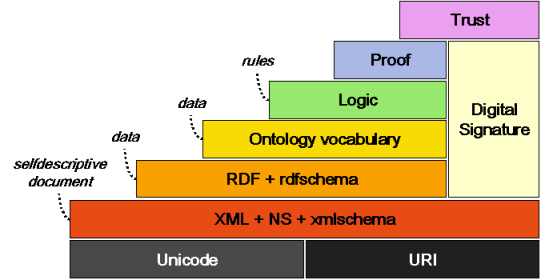
\includegraphics[scale=0.7]{images/semantic_web}}
\label{fig:semantic_web}
\caption{Semantic Web - vrstvy.\\Zdroj: \cite{semanticweb}}

\end{figure}

XML vrstva zaručuje, že môžeme spájať Sémantický web s inými normami, založenými napríklad na XML, ktorá je rozšírená a podporovaná a RDF dáta sa v nej dajú dobre prenášať, spracovávať a uchovávať. Toto je už ale pre dnešné časy neštandartné a viac sa využíva výmena dát pomocou JSON formátu. 


RDF je metóda popisovania vecí pomocou vzťahu medzi dvoma objektami. Napríklad koncepčne povedané ''Jožko má jablko'' je zadefinovaním spojenia medzi objektami ''Jožko'' a ''jablko'' pomocou vzťahu ''má''.
Toto spojenie je známe ako triplet, ktorý je základnou stavebnou jednotkou sémantického webu. 


RDF je aj názov slovníka, ktorý obsahuje množinu preddefinovaných termínov. Tieto termíny sú všeobecne používané na popis dát. Napríklad obsahuje najzákladnejšiu vlastnosť pre objekty a to vlastnosť typu objektu -- \textit{rdf:type}. 


RDFS je taktiež slovník. V RDF slovníku máme termíny, ktoré nám pomáhajú určovať definície a popisy jednotlivých objektov. V RDFS získavame možnosť popisovať triedy. Pokiaľ si zoberieme triedu ''Osoba'' a triedu ''Žena'', vieme pomocou RDFS slovníka zadefinovať vzťah podtriedy vlastnosťou ''rdfs:subClassOff''. Vďaka slovníkom RDF a RDFS môžeme tvoriť detailné popísanie našich dát.


Ontológia je v našom ponímaní synonymom k slovu slovník. Slovník RDFS môže byť použitý na tvorbu vlastnej ontológie. Sú v nej definované 


Vďaka takejto reprezentácii dát je možné písať pravidlá, ktoré má daný súbor dát spĺnať. Vďaka logickej vrstve vieme napríklad zadefinovať pravidlá ako: Všetky objekty typu ''Muž'' a ''Žena'' sú zároveň typom ''Osoba'' alebo Množina objektov s typom ''Muž'' je disjunktná s množinou objektov ''Žena''. Tieto pravidlá slúžia na kontrolu konzistentnosti našich dát.


\assignment{MH: \UP Toto trochu povrchne: (1) Ucelom SW nie je vyssia pouzitelnost webu (to je nepresne), ale je to lepsia pristupnost informacii publikovanych na webe pre strojove spracovanie. (2) Ak chces popisovat vrstvy SW podla tohto diagramu, bolo by dobre keby si popisal vsetky vrstvy -- U XML by som sa obmedzil na to, ze je to proste dobry format pre textovu reprezentaciu dat v suboroch a pre ich vymenu medzi softvermi -- toto vsak uz je dnes prekonane, uz vymiename SW data aj ako JSON, embedujeme ich do HTML5 (chcelo by to poznamku) -- O RDF a RDFS si vlastne nic uzitocne (z coho citatel nieco vyrozumie) nepovedal -- no a ostatne vrstvy si uplne preskocil\\
MH: Toto si menil? Zda sa mi, ze trochu asi aj ano, ale o tych dalsich vrstvach si nic nenapisal\\
MR: Popisane su uz aj dalsie vrstvy, mali by byt uz hotove}



Text uvedený nižšie popisuje niekoľko technológií, ktoré sú potrebné pre tvorbu sémantického webu.

\section{Linked Data}

\assignment{MH: \DOWN Tato sekcia je celkom fajn ale chybalo mi trochu
premostenie od SW -- linked data bola iniciativa, ze ked uz SW formaty mame,
podme v nich aj data zverenjnovat}


Linked Data \cite{linkeddata} alebo prepojené dáta, je metóda zverejňovania štrukturovaných dát. Ich hlavným cieľom je poprepájať existujúce databázy (primárne písané v RDF formáte), medzi rôznymi údajmi a umožniť ľuďom zdielať štrukturované dáta na webe pomocou HTML. Časť vízie do budúcna je, aby sa Internet stal globálnou databázou. Princípy prepojených dát prvýkrát načrtol Tim Berners-Lee. Popísal 4 pravidlá pre zverejňovanie dát na webe:
\begin{enumerate}
  \item používať URI ako názvy objektov, ktoré sú identifikátormi informácie, jej umiestnenia a ďalších vlastnotí,
  \item používať HTTP URI, aby si ich ľudia vedeli pozrieť,
  \item uvádzať informácie o tom, čo názov identifikuje pri vyhľadávaní pomocou otvorených štandardov, ako sú napríklad RDF alebo SPARQL,
  \item pri publikovaní údajov na webe, zahrnúť odkazy aj na iné URI, aby sa dalo objavovať viac vecí.
\end{enumerate}
Sú známe aj ako Princípy prepojených dát.

\assignment{MH: Tu mi chyba informacia, ze sa tato inciativa ujala, a ze vdaka
tomu vznikla na webe tzv. siet prepojenych dat, ktora obsahuje obrovske mnozstvo
datovych zdrojov a nieco viac o tej sieti.}


\section{Resource Description Framework (RDF)}

RDF \cite{rdf} je štandartný model na zakódovanie metadát a ďalších informácií. Je to taktiež formát, ktorý bol navrhnutý a štandardizovaný na reprezentáciu dát pre sémantický web. Zdroje týchto dát sú väčšinou webové zdroje, ktoré môžu byť čokoľvek, napríklad dokumenty, ľudia, fyzické objekty, atď. Taktiež poskytuje spoločný framework na vyjadrenie informácií a možnosť zdieľať ich medzi softvérmi, bez straty ich hodnoty. Dáta sa uchovávajú v Triple Store databázach, ktorých formát je striktne daný. Výhodou je, že dáta môžu byť spracované aj softvérmi, pre ktoré dané dáta neboli vytvorené.

\assignment{MH: \UP Na co RDF sluzi sa uz citatel dozvedel v skorsich castiach
(ked to tam lepsie ozrejmis). Niektore veci, ktore tu \UP pises su nepresne
(napr. to o tych metadatach a ``dalsich informaciac'' alebo o zdrojoch. Tiez o Triple Stores predbiehas, budes o tom pisat neskor\ldots Asi by som to tu skratil a len by som nadviazal, ze RDF je zakladny datovy format pre SW a tu ho popiseme\ldots}

\assignment{MH: \DOWN Zvysok ide dobrym smerom, je to presne to, co by som si predstavoval, ze tu budes pisat, len by som to chcel vidiet mozno trochu pomenej, podrobnejsie, systmatickejsie prebrate\ldots Na vacsom priestore, mozno postupne ten priklad budovat\ldots Vysvetlit na nom vsetky zakladne moznosti RDF}


RDF súbor je taký dokument, ktorý ukladá RDF grafy do špecifického formátu serializácie pre RDF, ako sú napríklad N-Triple, TURTLE, RDF/XML a mnohé ďalšie. RDF bol postavený na myšlienke vytvárať údaje vo forme predmet-predikát-objekt, ktorý sa volá triplet. Triplet je základná stavebná jednotka akejkoľvek množiny dát zapísaných v RDF. Tieto údaje sú reprezentované ako orientované grafy. Predmet a objekt predstavujú vrcholy a predikát je orientovaná hrana medzi nimi. Predmet môže byť použítý aj ako objekt v inom triplete. Týmto spôsobom sa triplety prepájajú a vzniká z nich grafová databáza. Predmet je vždy definovaný ako URI a popisuje zdroj informácie. Objekt môže byť taktiež nejaké URI popisujúce zdroj, ale taktiež to môže byť primitívna hodnota, ako napríklad string, integer, date, atď. Predikát popisuje, aký vzťah alebo rola medzi predmetom a objektom existuje. Predikát je vždy reprezentovaný ako URI, ktoré pochádza z ontolológií (kolekcie viacerých URI).


Na uľahčenie ukladania a čitateľnosti dát sa využívajú takzvané prefixy, ktoré sú preddefinovaním základných URI, do ktorých sa dodáva zvyšná hodnota URI pomocou dvojbodky, ako je to uvedené v nasledujúcom príklade a graficky znázornené v obrázku 2.2.
\begin{verbatim}
@prefix  rdf: <http://www.w3.org/1999/02/22-rdf-syntax-ns> .
@prefix	 dbr: <http://dbpedia.org/resource/> .
@prefix 	 dbo: <http://dbpedia.org/ontology/> .
@prefix  dbp:<http://dbpedia.org/property/> .

dbr:Bratislava dbo:highestPlace dbr:Devínska_Kobyla .
dbr:Bratislava rdf:type dbo:City .
dbr:Bratislava dbo:country dbr:Slovakia .
dbr:Devínska_Kobyla dbo:locatedInArea dbr:Slovakia .
dbr:Slovakia dbp:drivesOn "right" .
dbr:Slovakia dbo:longName "Slovak Republic"@en .
\end{verbatim}

\begin{figure}[h]
\makebox[\textwidth]{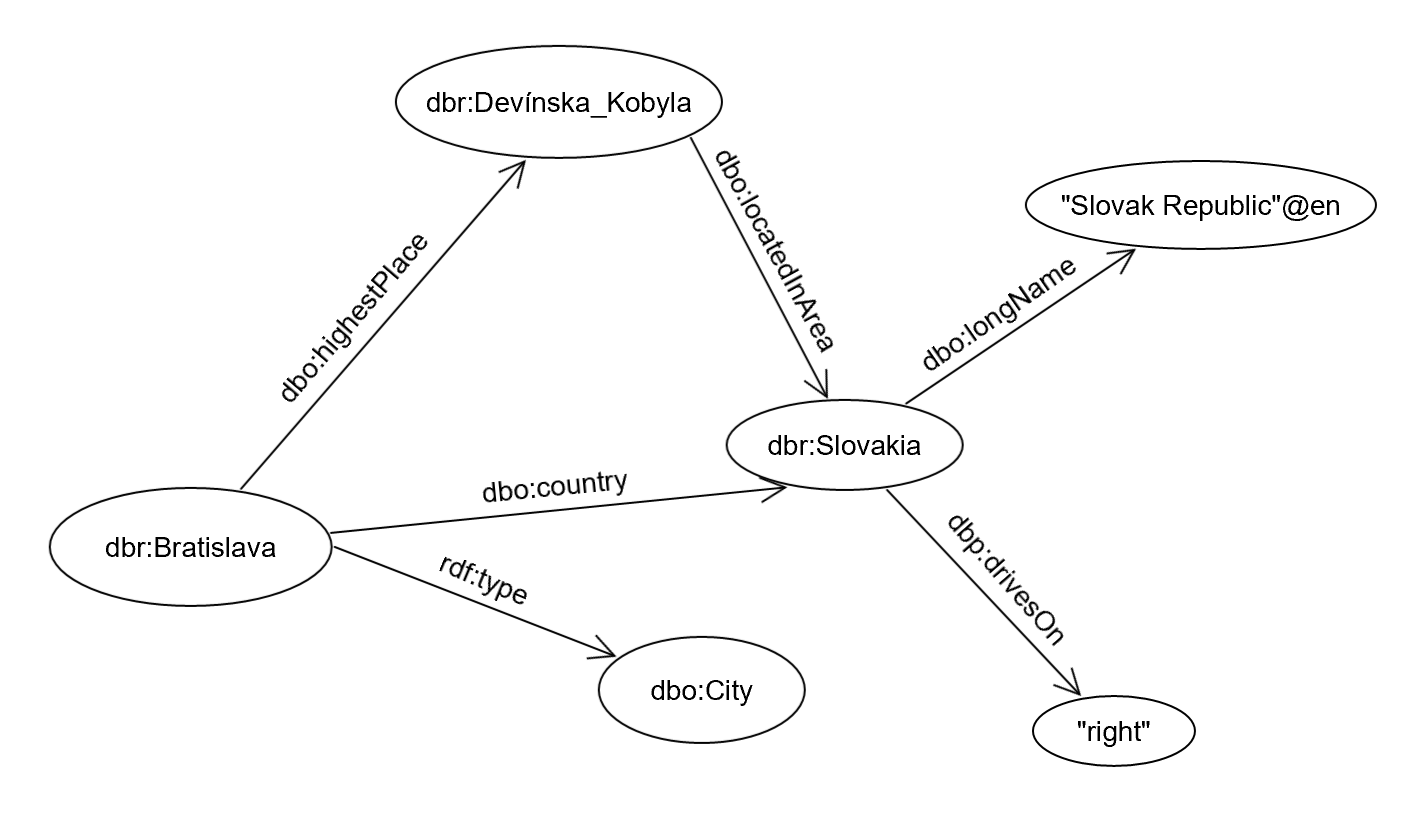
\includegraphics[keepaspectratio=true,scale=0.7]{images/triple_example}}
\label{fig:semantic_web}
\caption{Príklad grafovej databázy.}
\end{figure}

\section{SPARQL}
SPARQL \cite{sparql} je dopytovací jazyk pre RDF databázy, ktorý umožňuje získavanie a manipuláciu s databázou. Bol vytvorený skupinou DAWG, ktorá je súčasťou W3C a je uznávaný ako kľúčová technológia sémantického webu. 


\quad Ak by sme porovnali SPARQL s dopytovacím jazykom pre relačné datábazy, napr. SQL, zistíme, že sú si podobné v kľúčových slovách, ako sú napr. SELECT, WHERE, FROM atď. SPARQL dopyt využíva trojice ako základný prvok, kde predmet, predikát alebo objekt môžu byť premenné. Dopyt sa robí nad dátovou kolekciou RDF, čo je množina dokumentov, patriaca pod určitý koncový bod - '\textit{endpoint}'. Je to dopytovací jazyk, ktorý z orientovaného ohodnoteného grafu zisťuje hodnoty jednotlivých vrcholov a hrán, ktoré sú výstupnými parametrami dopytu.

\begin{verbatim}
@prefix	 dbr: <http://dbpedia.org/resource/> .
SELECT ?predicate ?object WHERE {
  dbr:Bratislava ?predicate ?object .
}
+------------------+---------------------+
| ?predicate       | ?object             | 
+------------------+---------------------+
| dbo:highestPlace | dbr:Devínska_Kobyla | 
| rdf:type         | dbo:City            | 
| dbo:country      | dbr:Slovakia        | 
+------------------+---------------------+
\end{verbatim}


Príklad dopytu nad databázou uvedenou vyššie, spúšťame nad endpointom DBPedia a výsledok je len zlomkom z toho, čo nám skutočne vráti: Chceme získať všetky údaje o Bratislave.


Okrem operácie SELECT poznáme aj ďalšie typy dopytov. ASK je dopyt, ktorý nám vracia pravdivostnú hodnotu pre daný dopyt. Vieme ním napríklad zistiť, či sa v našom grafe nachádza mesto Bratislava. Taktiež poznáme dopyt DESCRIBE, ktorý vracia RDF graf opisujúci jednotlivé vlatnosti výsledných hodnôt dopytu. Ako posledný typ dopytu je CONSTRUCT, ktorý vracia nový RDF graf podľa predlohy vytvorenej v hlave dopytu.

\chapter{Ontológie}

\assignment{MH: Predpokladam, ze o ontologiach budeme pisat o znacny kus viac a
podrobnejsie\ldots Mozes vychadzat z mojej prednasky ale tiez napr z uvodnej
kapitoly \emph{Handbook on Ontologies}}


Výraz ontológia \cite{ontology} pochádza z gréckeho slova kde '\textit{ontos}' znamená existencia a '\textit{logos}' znamená veda. Ontológia v informatike je uceleným popisom pojmov v určitej oblasti záujmu. Obsahuje určitú klasifikáciu údajov do hierarchicky usporiadaných kategórií a množinu odvodzovacích pravidiel, pomocou ktorých je možné z faktov odvodiť nové skutočnosti. Prostredníctvom ontológií je možné vytvárať spojenia, vykonávať analýzu údajov a sprostredkovať výhody webu obohateného o sémantiku. 


Jej cieľmi je zadefinovanie a zdieľanie jednotného zápisu informácií pre danú doménu. Ak napríklad viac stránok využíva na popis pojmov takúto zadefinovanú ontológiu, vedia boti získať a vyhľadávať viac dát o hľadanej informácii.


Taktiež je jej cieľom opätovné použitie ontológie, napríklad ak máme dobre zadefinovanú ontológiu, môžu ontologický inžinieri doplniť do našej ontológie ďalšie vlastnosti a tým by základ ontológie bol rovnaký ale bol by rozšírený o určité dáta, podľa potreby ontologických inžinierov.


%\assignment{MH: nerozumiem co myslis pod \uv{vytvárať spojenia v prirodzenomjazyku} a tiez tvrdenie \uv{sprostredkovať výhody webu obohateného o sémantiku} je velmi abstraktne neviem celkom prist na to co si tym asi myslel}

\section{Základné pojmy}
Ontológia sa skladá zo základných stavebných prvkov \textit{Trieda}, \textit{Entita}, \textit{Atribút}, \textit{Vzťah}. 


\textbf{Triedy} alebo typy definujú skupiny alebo množiny objektov. Triedy majú hierarchickú štruktúru zloženú z ich podtried. Každá podtrieba spĺňa vlastnosti nadtriedy a môže byť rozšírená o vlastné vlastnosti.


\textbf{Entity} sú individuálne inštancie nejakej nami zadefinovanej triedy. Ak by sme mali entitu \textit{Bratislava}, a triedy \textit{Mesto} a \textit{Hlavné mesto}, kde \textit{Mesto} je podtriedou \textit{Hlavné mesto}, tak nám z ontológie vyplýva, že ak je entita \textit{Bratislava} individuálnou inštanciou triedy \textit{Hlavné mesto}, tak je aj individuálnou inštanciou triedy \textit{Mesto}.

%\minor{MH: $\uparrow$ \emph{Jablko} nie je velmi dobry priklad na entitu, kedze vacsinou ho uvazujeme ako triedu (a teda podtriedu triedy Ovocie)\\
%MR: upravene na Bratislava, to sa da lahko tvorit.}


\textbf{Atribúty} sú vlastnosti \textit{Tried} a \textit{Entít} a môžu niesť rôzne informácie o danom objekte. \textit{Atribúty} môžu mať rôzne hodnoty, ako reťazec, číslo, dátum alebo pravdivostnú hodnotu. Ak by sme si zobrali predchádzajúcu entitu \textit{Bratislava}, jej číselná vlastnosť môže byť napríklad počet obyvateľov.

%\assignment{MH: $\uparrow$ Je pomerne nezvycajne aby mali atributy ako hodnotu inu premennu}

\textbf{Vzťahy} sú najpodstatnejšou súčasťou ontológie. Poskytujú prepájanie jednotlivých entít. Je to jednosmerné spojenie, ktoré určuje vzťah, v akom sú dve dané triedy. Tým vznikne triplet \textit{trieda:vzťah:trieda}. Medzi triplet sa radí aj trojica \textit{trieda:atribút:hodnota}. Väzby sa zvyknú definovať aj inverzne. Z logického hľadiska sú vzťahy axiómami. Pokiaľ máme triedu \textit{Krajina} a \textit{Hlavné mesto}, tak by vzťah mohol vyzerať nasledovne: Krajina:má:Hlavné mesto.


\textbf{TBox} je množina definícií tried a ich vzťahov medzi nimi. V množine je obsiahnutá znalosť taxonómie tried, taktiež v nej môže byť zadefinovaná disjunktnosť jednotlivých tried, vymenovanie konkrétnych entít obsiahnutých v danej triede, reštrickie pre jednotlivé triedy a ich vzťahy.


\textbf{ABox} je množina znalostí o jednotlivých entitách.

%\assignment{MH: $\uparrow$ nazov \emph{vazby} je velmi exoticky. Ak ti ide o object properties, pouzil by som slovo \emph{vztahy}.}
%\assignment{MH: $\uparrow$ to co je \emph{triplet} by si mal zadefinovat vyssie, kde pises o RDF.}
%\assignment{MH: $\uparrow$ Co su \uv{objekty tried}? Kusok vyssie si si pre objekty zvolil nazov \emph{entity}, mal by si ho teda pouzivat. Ak ti ide o vztahy medzi triedami, ako napr. vztah podtriedy a nadtriedy, v RDF je to sice vyjadrene pomocou vlasntosti, ale z logickeho hladiska to chapeme ako \emph{axiom}}

Ontológia má veľa vlastností, ktoré musia byť dodržané. Každý prvok musí byť jasne indetifikovateľný. Taktiež zakazuje zapisovanie duplicitných dát, čo nám zaobstará vlastnosť efektívneho ukladania informácií, kde to môže nie len uľahčiť vyhľadávanie ale aj zredukovať obsah pamäti na disku. 

\assignment{MH: $\uparrow$ Neviem, ci zrovna tieto vlastnosi ontologii su tie najpodstatnjsie, a teda treba ich spominat na tomto mieste.\\
MR: Urcite by som ich spomenul nakolko existuje urcite vela duplicitnych dat a je to vyhoda oproti SQL kde kazdy zaznam v ciselniku ma unikatne IDcko ale u nas je to predstavovane iba entitou.}

\section{Využitie ontológií}

Ontológie sa začali využívať najmä v organizáciách, ktoré sa špecializovali na umelú inteligenciu. Neskôr sa to rozšírilo aj do bežne používaných aplikácií. Napríklad firma Amazon používa ontológie na kategorizovanie tovaru v ich elektronickom obchode.

\assignment{MH: $\uparrow$ Vies to dolozit nejakou referenciou? Skade mas tu informaciu...}


%Na zápis týchto ontológií sa používa niekoľko jazykov, kde najznámejším je asi Resource Description Framework (RDF), ktorý je rpimárne určený na využitie vo webových stránkach, pre hľadanie informácií strojmi. 
Ontológie si našli uplatnenie aj v medicínskej oblasti a to napríklad SNOMED, čo je najväčším viacjazyčným medicínskym slovníkom na svete. 

\assignment{MH: Cituj SNOMED, najdi vhodny zdroj cez Google Scholar}

Taktiež sa s ním stretávame každodenne pri vyhľadávaní na stránke Google, kde ako bočný panel sú zobrazené informácie o vyhľadávanom objekte (~\ref{fig:semantic_web}). Tieto dáta je možné zobraziť preto, lebo výsledkom takéhoto panelu je vyhľadávanie informácií na webovej stránke, ktorá obsahuje sémantické dáta.

\begin{figure}[h]
\makebox[\textwidth]{
\includegraphics[keepaspectratio=true,scale=0.7]{images/onto_screen}}
\label{fig:semantic_web}
\caption{Príklad bočného panelu vo vyhľadávači Google.}
\end{figure}

Schema.org \cite{schemaOrg} je taktiež ontologickým riešením, ktorej cieľom je vytvárať, udržiavať a propagovať schémy štrukturovaných údajov na internete, internetových stránkach alebo e-mailových správach. Poskytuje zdieľanú slovnú zásobu, ktorú môžu tvorcovia internetových stránok používať na označenie a popis jednotlivých elementov na stránke. Týmto popisom rozumejú vyhľadávacie nástroje ako Google, Microsoft a Yahoo!. Viac ako 10 miliónov internetových stránok používa Schema.org na popisovanie svojich stránok a e-mailových správ.

\assignment{MH: $\uparrow$ mozes referenvovat aj priamo web, ale odnorny clanok o Schema.org je: Guha, R.V., Brickley, D. and Macbeth, S., 2016. Schema. org: evolution of structured data on the web. Communications of the ACM, 59(2), pp.44-51.}

\section{Web Ontology Language}
Jazyk Web Ontology Language alebo OWL slúži na vytváranie a definovanie inštancií webových ontológií. Poskytuje nástroje na popis tried, vlastností a ich samotných inštancií. Oproti klasickým jazykom poskytje možnosť, špecifikovať logické vlastnosti jednotlivých objektov vyskytujúcich sa v ontológií, čo znamená, že dokáže popísať aj fakty, ktoré v ontológií nie sú definované priamo, ale sú spojené logickými vlastnosťami. Napríklad, ak máme osoby Janka, Martin a Jozef, kde Janka je rodičom Martina a Jozef je rodičom Janky, pomocou OWL vieme definovať, že Jozef je starým rodičom Martina, pričom nepotrebujeme vlastnosť popisujúcu tento vzťah priamo.

\assignment{MH: $\uparrow$ Tomuto nerozumiem}


%\subsection{Druhy OWL}
%Jazyk OWL poskytuje 3 podjazyky, ktoré sú použitľné v rôznych situáciách.


%OWL 2 EL je odporúčaný pre ontológie, ktoré definujú veľké množstvo tried a/alebo vlastností. Podporuje základné definície tried, disjunktné triedy, ekvivalenciu vlastností a tried, tranzitivitu vlastností, reflexné objekty, obmedzenie domény a rozsahu objektov. Taktiež dokáže definovať obmedzenia tried ako existenciálne obmedzenie, obmedzenie týkajúce práve jedného objektu alebo hodnoty z viacerých.


%OWL 2 QL


%OWL 2 RL je zameraný na aplikácie, ktoré potrebujú škálovateľnosť uvažovania bez toho, aby obetovali expresívnu silu jazyka. 


%Každý, kto sa rozhodne vyvýjať ontológiu použitím OWL, by mal zvážiť, ktorý typ je najlepší pre danú ontológiu. Najmä treba zvážiť aké obmedzenia je potrebné pre ich ontológiu definovať. 


\subsection{Syntax}
\assignment{MH: (1) Man syntax je zrozumitelnejsia (2) moc daleko si nedosiel... Na zac. sa detailne venujeme nie prilis podstatnym veciam}
Na popis jednotlivých možností budeme používať Manchester syntax, ktorá poskytuje zrozumiteľnejšiu syntax pre čitateľa.

\assignment{MH: $\uparrow$ Toto nie je Man syntax, toto je tzv. Functional Style Syntax}

Ako prvé si zadefinujeme priradenia objektov k jednotlivým triedam. Objekty môžu mať pridelených viac tried.
\begin{verbatim}
ClassAssertation( :Osoba :Janka )
ClassAssertation( :Žena :Janka )
ClassAssertation( :Osoba :Martin )
ClassAssertation( :Muž :Martin )
ClassAssertation( :Osoba :Jozef )
ClassAssertation( :Muž :Jozef )
\end{verbatim}


Ako si možeme všimnúť vyššie, Janke sme museli priradiť dve triedy. Týmto triedam ale vieme vytvoriť hierarchickú štruktúru.
\begin{verbatim}
SubClassOf( :Žena :Osoba )
SubClassOf( :Matka :Žena )
\end{verbatim}


Niekedy môžeme mať dve rôzne definície tried, ktoré však predstavujú tú istú osobu. Takéto triedy sa volaú ekvivaletné a vieme ich definovať nasledovne:
\begin{verbatim}
EquivalentClasses( :Človek :Osoba )
\end{verbatim}

\assignment{MH: $\uparrow$ nepredstavuju \emph{tu istu osobu} ale tu istu triedu, entitu, koncept, ... Tu isty osobu by mohli predstavovat 2 individualy}


Ďalej si vieme zadefinovať vlastnosti objektov. Tieto vlastnosti vieme definovať buď pozitívne, kedy objekt danú vlastnosť má, alebo negatívne, kedy objekt danú vlastnosť s druhým objektom mať nemôže.
\begin{verbatim}
ObjectPropertyAssertion( :jeMatkou :Janka :Martin )
ObjectPropertyAssertion( :jeOtcom :Jozef :Janka )

NegativeObjectPropertyAssertion( :jeOtcom :Jozef :Martin )
\end{verbatim}


Veľmi podobne vieme definovať aj dátové priradenia k jednotlivým objektom.
\begin{verbatim}
DataPropertyAssertion( :máVek :Janka "38"^^xsd:integer )

NegativeDataPropertyAssertion( :máVek :Jozef "10"^^xsd:integer )
\end{verbatim}


Tieto vlastnosti môžu mať taktiež hierarchickú štruktúru.
\begin{verbatim}
SubObjectPropertyOf( :jeMatkou :jeRodičom )
SubObjectPropertyOf( :jeOtcom :jeRodičom )
\end{verbatim}

\assignment{MH: $\uparrow$ \uv{Tieto vlasntosti}? Hovoril si nieco o vlastnostiach? Vlastne si o nich nic dokopy nepovedal... Heirarchu roli a vztah podvlasntnosti treba lepsie vysvetlit}


Týmto vlastnostiam vieme definovať ich domény a rozsah, ktoré definujú, aké hodnoty môžu jednotlivé vlastnosti nadobúdať, a s akým objektom môžu byť tieto vlastnosti pridelené.
\begin{verbatim}
ObjectPropertyDomain( :jeRodičom :Osoba )
ObjectPropertyRange( :jeRodičom :Osoba )
ObjectPropertyDomain( :jeMatkou :Žena )
ObjectPropertyRange( :jeMatkou :Osoba )
ObjectPropertyDomain( :jeOtcom :Muž )
ObjectPropertyRange( :jeOtcom :Osoba )

DataPropertyDomain( :máVek :Osoba ) 
DataPropertyRange( :máVek xsd:nonNegativeInteger ) 
\end{verbatim}


Ďalej vieme definovať inverznosť vlastností. Napríklad pokiaľ máme vlastnosť je rodičom, jej inverzná vlastnosť je je dieťatom.
\begin{verbatim}
InverseObjectProperties( :jeRodičom :jeDieťaťom )
InverseObjectProperties( :jeMatkou :máMatku )
InverseObjectProperties( :jeOtcom :máOtca )
\end{verbatim}


Niektoré vlastnosti by sme nechceli definovať iba jednosmerne ale aj obojsmerne. Takouto vlastnosťou sa myslí symetrická vlastnosť.
\begin{verbatim}
SymmetricObjectProperty( :jePríbuzný )
\end{verbatim}


Jazyk OWL poskytuje definície rôznych obmedzení. Ako prvou si spomenieme disjunktnosť jednotlivých tried, kde jednotlivé objekty nemôžu patriť do oboch tried zároveň.
\begin{verbatim}
DisjointClasses( :Muž :Žena )
\end{verbatim}


Ďalším obmedzením je definovanie, či je konkrétny objekt tým istým alebo iným objektom.
\begin{verbatim}
DifferentIndividuals( :Janka :Martin )
DifferentIndividuals( :Janka :Jozef )

SameIndividual( :Martin :Maťo )
\end{verbatim}


Taktiež vieme definovať objekty, ktoré spadajú pod rovnakú triedu, pokiaľ spĺňajú určité vlastnosti. Napríklad, všetky ženy, ktoré sú zároveň rodičom, sú aj matkou. Vieme povedať aj to, že všetky objekty, ktoré sú buď matkou alebo otcom, sú zároveň aj rodičom.
\begin{verbatim}
EquivalentClasses(
  :Matka 
  ObjectIntersectionOf( :Žena :Rodič )
) 

EquivalentClasses(
  :Rodič 
  ObjectUnionOf( :Matka :Otec )
) 
\end{verbatim}


Ďalej vieme definovať existenčné obmedzenia na objekt a vlastnosti. Napríklad, každý rodič musí mať dieťa.
\begin{verbatim}
EquivalentClasses(
  :Rodič 
  ObjectSomeValuesFrom( :jeRodičom :Osoba )
)
\end{verbatim}

\assignment{MH: $\updownarrow$ obmedzenia treba aj vysvetlit. Ty si to vysypal z rukava, predpokladas, ze citatel uz vie co to je, aku to ma semantiku, a len si uviedol syntax... Treba vyscvetlit. Vseobecne obmedzenie skor nazyvame hodnotove obmedzenie}

Podobne ako existenčné, si vieme definovať aj všeobecné obmedzenie. Napríklad rodiča, ktorý ma iba chlapcov si zadefinujeme nasledovne:
\begin{verbatim}
EquivalentClasses(
  :RodičIbaChlapci 
  ObjectAllValuesFrom( :jeRodičom :Muž )
)
\end{verbatim}


V príklade vyššie nám však toto obmedzenie nezaručuje, že daný rodič musí mať dieťa. Na takéto zabezpečenie sa využíva existenčné a všeobecné obmedzenie zároveň. Týmto obmedzením hovoríme, že musí mať minimálne jedno dieťa, ktoré je chlapcom a zároveň všetky jeho deti sú chlapci.
\begin{verbatim}
EquivalentClasses(
  :RodičIbaChlapci 
  ObjectIntersectionOf(
    ObjectAllValuesFrom( :jeRodičom :Muž )
    ObjectSomeValuesFrom( :jeRodičom :Muž )
  )
)
\end{verbatim}



\assignment{MH: Toto nema nejake vhodne ukoncenie. Konci odseknutim. Aspon povedz, ze OWL ma este dalsie uzitocne konstruktu a nejake priklady este vymenuj bez vacsieho vysvetlvoania, napr. cardianlity restrictions, nominaly, ...}


\chapter{Existujúce ontologické riešenia}
Množstvo kyber útokov v dnešnej dobe narastá závratnou rýchlosťou, čo značí, že dnešné spôsoby a metódy ochrany nie sú dostatočné, a preto je potrebné sa zamyslieť nad novými spôsobmi ochrany. Jeden z prístupov by mohol byť založený práve na ontológiách. Ontológie a systémy postavené nad nimi majú výhodu sémantiky, ktorá je schopná rozlišovať situácie kedy je počítačový systém normálny alebo škodlivý.


Problém, s ktorým sa však potýkame je ten, že neexistuje jednotný formát zápisu údajov. Väčšina nástrojov, ktoré v dnešnej dobe existujú, majú vlastné štandardy. Keďže tieto štandardy sú prevažne rozdielne, nedá sa ich prepájať a využívať efektívne. Tento problém by mohol byť taktiež vyriešený vďaka ontologickému riešeniu. Tým pádom by sme vedeli mať také dáta, ktoré dokážu stroje nielen prečítať, ale zároveň aj pochopiť. 
 

Ontologiký prístup taktiež poskytuje jednoduchšiu rozšíriteľnosť už existujúcej ontológie, a tým sa dá vytvárať presnejší popis záznamov.


Vďaka URI reprezentácií jednotlivých entít, ktoré sú používané ako identifikátory jednotlivých objektov, nemôže nastať problém nepochopenia dát, ako k tomu môže doochádzať v ľudskej reči. Napríklad ak by sme povedali slovo \textit{koruna}, nikto nevie, či máme na mysli korunu stromov alebo kráľovskú korunu. Avšak vďaka atribútom vieme toto slovo lepšie pochoiť, keďže nám ho atribúty bližšie definujú.

\minor{MH: $\uparrow$ Tento text sa skor hodi do uvodu, pripadne cast do casti kde opisujes ontologie. Tuto kapitolu by som ocakaval, ze otvoris nejak zhruba odtialto $\downarrow$ (Akoze toto $\uparrow$ sa uz citatel (mal) dovediet niekde predtym a je zbytocne to tu opakovat\ldots)}

V súčastosti existuje veľa rôznych štandardov a ontologických riešení pre doménu kyber bezpečnosti, avšak veľa z nich už ani nie je vyvýjaných. Organizácie, ktoré vyvýjali tieto ontológie, buď stratili o ďalší vývoj záujem, alebo už len nezverejňujú svoje pokroky v danej doméne, teda prešli na closed-source systém.


V nasledujúcich kapitolách si povieme niečo o zaužívaných štandardoch, základnom modeli, z ktorého vychádzame a podľa ktorého posudzujeme, či je daná ontológia dobrá. Taktiež rozoberieme existujúce riešenia v doméne kyber bezpečnosti.

\section{CTI model}
Cyber Threat Intelligance model \citep{MavroeidisB17} (CTI model) má za cieľ objasňovať rôzne typy informácií, ktoré potrebujú organizácie zhromažďovať o kybernetických hrozbách. Cieľom modelu je jednotne definovať a podrobne popísať okruhy v danej doméne. Výhodou takéhoto modelu je zlepšenie schopností pri prevencii, detekcii a reakcii na bezpečnostné hrozby.


Tento model bol vyvinutý so zámerom, aby slúžil ako predloha pre ontologické riešenia, nakoľko autori zahrnuli fakt, že ontologické riešenia sú najlepšie pri publikovaní a zdieľaní dát, a sú strojovo čitateľné vďaka typu reprezentácie.


Model zahŕňa informácie o autorovi útoku, motivácie a ciele útoku, stratégiu akou je útok vedený, aké technológie a postupy používa, ktorým základným vzorcom útoku sa riadi, aké slabiny jednotlivé útoky využili, aké atomické indikátory dokážu predpovedať útok a akú cieľovú skupinu útok postihuje.


V nasledujúcich častiach popíšeme niektoré okruhy z obr. 4.1, ktorý znázorňuje jednotlivé prvky modelu.


\begin{figure}
\makebox[\textwidth]{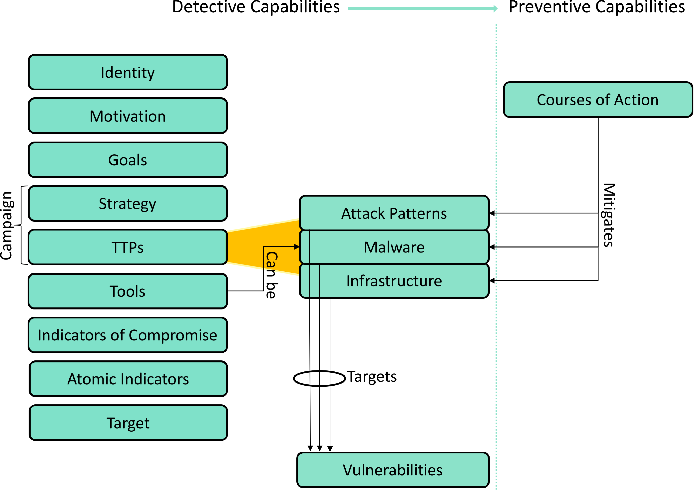
\includegraphics[scale=0.5]{images/cti-model}}
\label{fig:semantic_web}
\caption{CTI model.\\Zdroj: \citep{MavroeidisB17}}

\end{figure}

\subsection{Identita}
Identita môže byť definovaná rôznymi typmi identifikátorov. Ak sa pozná presná totožnosť osoby alebo organizácie, ktorá útok iniciuje, identifikátorom je názov osoby alebo spoločnosti.


Pokiaľ takýto identifikátor nevieme určiť, prideľujeme im anonymnú identitu, ktorú následne vieme spájať vyhodnotením útoku. Pokiaľ zoberieme do úvahy všetky ostatné časti CTI modelu a vyhodnotíme zhodujúce sa časti, vieme povedať, za ktoré útoky zodpovedá rovnaká osoba alebo organizácia.



\subsection{Kampaň}
Kampaň popisuje samtotný útok z dvoch pohľadov. Netechnický, ktorý je reprezentovaný stratégiou a technický, ktorý definuje taktiky, techniky a procedúry využívané v útoku.

\subsubsection{Stratégia}
Stratégia predstavuje netechnický popis útoku na hornej úrovni. Pokiaľ si zoberieme nejakého útočníka, tak tento útočník zvyčajne dosahuje ciele útoku viacerými spôsobmi a stratégia definuje, čo a ako je potrebné pozorovať.

\subsection{Zraniteľnosť}
Zraniteľnosti definujú slabiny systému. Tieto slabiny môžu byť definované rôznymi stavmi zariadenia, ako napríklad, ktoré systémy bežia, ale môžu predstavovať aj nastavenia rôznych aplikácií, napríklad rôzne prístupové nastavenia a povolenia pre webové prehliadače. Taktiež môžu popisovať rôzne funkcie, ktoré umožňujú vykonávať jednotlivé systémy, ako napríklad spúšťanie rôznych príkazov ktoré ovplyvňujú a menia systémové nastavenia zariadenie.

\subsubsection{TTP}
Taktiky, techniky a procedúry (TTP) sa zamieravajú na dáta čitateľné strojmi. Popisujú spôsoby útoku z hľadiska toho čo chcú dosiahnuť a ako to robia.


\textbf{Vzorec útoku} je jedným z hľadisiek TTP. Definuje akým spôsobom je útok použitý. Napríklad sa tu nachádzajú rôzne úpravy názvov súborov, rôzne prenastavenie časovania a stavov zariadenia, atď. 


\textbf{Malware} je taktiež hľadisko z TTP. Definuje typ softvéru, ktorý sa vkladá do systému s úmyslom poškodiť cieľ útoku z hľadiska dôvernosti, integrity alebo dostupnosti. Medzi typické malware patrí vírus, trójsky kôň, červ, metódy tajných vstupov, spyware, atď.


Každý okruh z TTP využíva niektoré zraniteľnosti systémov.


\subsection{Indikátor}
Indikátory predstavujú množinu rôznych vlastností zariadenia, kedy je zariadenie náchylné na útok. Tieto indikátory popisujú rôzne nastavenia zariadenia, jeho technické parametre alebo nainštalovaný softvér a vďaka nemu sú schopné definovať rôzne útoky.


\textbf{Atomické indikátory} sú najpremenlivejšie ukazovatele, nakoľko sa po čase menia. Napríklad, ak niektoré útoky prebiehajú z určitej IP adresy, tak táto adresa sa môže časom zmeniť. Tieto typy dát môžu pomáhať pri identifikovaní útočníka iba v určitom čase.


\subsection{Nástroj}
Nástroje sú pomôcky, ktoré útočníci inštalujú v zariadení obete. Väčšinou zahŕňa špecializovaný softvér priamo určený na spôsobenie škôd, ako napríklad vzdialené vykonávanie procesov alebo sieťové skenovanie. Taktiež môže byť použitý pre zabránenie detekcie útoku inými systémami.


\subsection{Zámer}
Zámer pomenováva koncový stav objektu útoku. Zámer nemusí byť vopred daný alebo zrejmý. Jednotlivé útoky môžu prebiehať aj s tým, že až počas útoku je zámer známy. Zámerom môže byť napríklad ukradnutie duševného vlastníctva, poškodenie systému, získanie kompromitujúcich dát a podobne.


\subsection{Cieľ}
Cieľom je myslená entita, na ktorú je útok namierený. Takouto entitou môže byť napríklad organizácia, štát alebo konkrétna osoba.

%\subsection{Útok}
%Samotný útok, by mal predstavovať konkrétny útok, ktorý už prebehol. Mal by zahŕňať mapovania na každú časť CTI modelu, ako aj nejaké statické informácie o útoku, napríklad čas útoku, ako daný útok dopadol a podobne.



\assignment{MH: Ano, urcite\\
MR: zahrnute, plus som sem vypichol casti ktore budeme popisovat z modelu a na ktore budem vyhodnococat UCO podrobne}

\section{Unified Cybersecurity Ontology}
Unified Cybersecurity Ontology \citep{SyedPFMJ16} alebo skrátene UCO je rozšírením pôvodného projektu Intrusion Detection System (IDS), ktorého tvorcom je rovnaká skupina. Spája viaceré bežne dostupné bezpečnostné štandardy používané v kybernetickej bezpečnosti. Prevažne pokrýva STIX, ktorý je najväčším a najkomplexnejším štandardom, pokrývajúcim najväčšiu časť kybernetickej bezpečnostnej domény ale taktiež pokrýva iné relevatné štandardy ako CVE4, CCE5, CVSS6, CAPEC7, CYBOX8, KillChain9 a STUCCO10.

%\minor{MH: $\uparrow$ Zrejme muslis \emph{pokryva} ine relevantne standardy? Ak nie, nerozumiem, v akom zmysle ich poskytuje?}

Aj keď je STIX najkomplexnejším štandardom a zjednocuje všetky informácie o kybernetických hrozbách, má tieto dáta uložené v XML súboroch, takže nepodporuje výhody inferencie v ontológiách, čo UCO poskytuje.

%\minor{MH: $\uparrow$ \emph{uvazovanie v ontologiach} nie je spravny slovensky vyraz pre reasoning -- skus napr. \emph{inferencia}}

Okrem týchto štandardov obsahuje aj mapovanie na všeobecné databázy, ako sú Google Knowledge Graph, DBPedia a Yago. Vďaka týmto mapovaniam je možné mať prístup k verejným databázam z rôznych domén záujmu.


Základnými triedami, využívanými v UCO sú: 
\begin{itemize}
\item \textit{Means} -- Čo je zamýšľané daným útokom.
\item \textit{Consequences} -- Dôsledky útoku.
\item \textit{Attack} -- Typ útoku.
\item \textit{Attacker} -- Kto je iniciátorom daného útoku.
\item \textit{Attack-Pattern} -- Vzorec útoku, podľa ktorého je útok riadený.
\item \textit{Exploit} -- K čomu útok slúži.
\item \textit{Exploit Target} -- K čomu slúži cieľ alebo výsledok útoku.
\item \textit{Indicators} -- Indikátor útoku.
\end{itemize}
Každá z týchto tried je mapovaná na už reálne existujúcu triedu v niektorom z vyššie uvedených štandardov, prevažne na STIX schému.


Ontológia UCO umožňuje analytikom zachytávať špecifické vedomosti o kybernetickej bezpečnosti pomocov termínov a tried z ontológie a taktiež umožňuje písať pravidlá, ktoré sa môžu použiť na odvodenie nových poznatkov.


Vývojári extrahovali dáta z National Vulnerability Database (NVD), ktorá je uložená v XML súboroch. Potom boli namapované na triple store DBPedia a dáta boli uložené na FUSEKI server, ktorý podporuje dopytovanie z rôznych zdrojov rovnako ako ich odvodzovanie.

\minor{MH: $\uparrow$ Zmienky o nejakych datach sa tu zjavia z cista-jasna... Doteraz sme hvorili stale o ontologii, nezapada to... (Mozno treba len previazat a upresnit?)}


\section{Integrated Cyber Analysis System}
Integrated Cyber Analysis System\citep{salem2015enabling} alebo ICAS je ontológia vytvorená pre TAPIO (Targeted Attack Premonition using Integrated Operational data) nástroj, ktorý je schopný extrahovať dáta z počítačov v jednej sieti do jedného sémantického grafu, a tým zjednoduší a urýchli prácu bezpečnostným tímom pri vyhľadávaní ohrození systému, čím by sa zvýšila prehľadnosť dát a tiež znížil dopad útoku. 


Samotná ontológia ICAS je veľmi komplexnou, nakoľko obsahuje približne 30 podontológií, kde každá sa špecializuje na inú oblasť v doméne informačnej bezpečnosti.

\minor{MH: $\uparrow$ vieme povedat, ze ci nejaka cast z toho je relevantna pre nas}

Nástroj TAPIO spolu s ontológiou ICAS bol vyvýjaný organizáciou DAPRA, ale dátum poslednej úpravy bol v roku 2017, teda podobne ako UCO sa jedná o projekt, ktorý už nie je aktuálny.

\assignment{MH: $\uparrow$ Tu by som bol opatrnejsi, tvrdit, ze nieco nie je aktualne, lebo posledny update bol pred 3 rokmi je zvlastne. Co ked pred troma rokmi to dotiahli uz do dokonalosti a teraz uz len pouzivaju?}

\section{STUCCO}
STUCCO \citep{stucco}, ktorej autorom je Iannacone at al., je ontológiou, ktorá je určená na prácu so znalostnými grafovými databázami. Jej základ tvoria scenáre použitia ľudskými používateľmi alebo automatizovanými strojmi. Obsahuje dáta z 13 rôznych štruktúr, ktoré majú rôzne formáty, a ktoré sú uložené v rôznych typoch databáz. 


STUCCO obsahuje dáta z nasledovných kategórií, do ktorých je rozdelená bezpečnostná doména. 
\begin{itemize}
\item Identita -- predstavuje totožnosť a vlastnosti útočníka.
\item Taktika technika a procedúry (TPP) -- Popisuje, čo daný útok robí a ako to robí.
\item Nástroje -- Aké nástroje sú potrebné pre úspešné vykonaie útoku.
\item Atomické indikátory -- Sem môžu spadať súbory, IP adresy, doménové mená atď. Nanešťastie tieto dáta majú krátku životnosť, nakoľko sa stále menia.
\end{itemize}

%%%%%%%%%%%%%%%%%%%%%%%%%%%%%%%%%%%%%%%%%%%%%%%%%%%%%%%%%%%%%%
%%%%%%%%%%%%%%%%%%%%%%%%%%%%%%%%%%%%%%%%%%%%%%%%%%%%%%%%%%%%%%
%%%%%%%%%%%%%%%%%%%%%%%%%%%%%%%%%%%%%%%%%%%%%%%%%%%%%%%%%%%%%%

\part{Vlastný prínos}
\chapter{Výskum a Analýza UCO}
\assignment{MH: Takze si to vlastne sem cele presnul a v Casti I uz o tom nie je ani zmienka? Tu by to malo byt uvedene sposobom, ze tu ju podrobne pispiseme a zanalyzujeme... Cize malo by to byt v Casti II vedene ako analyza UCO, nie jej len popis\\
MR: Done\\
MH: Namiesto $\downarrow$ \uv{popiseme a budeme porovnavat} napise \uv{podrobne analyzujeme a vyhodnocujeme vzhladom na}.. Nech je to este jasnejsie.\\
MR: Done\\
MH: Len uz v prvej vete ide o UCO? Ano, nie je to jasne, ked je tam len citacia. Tiez by tu mohol byt jej nazov, nie len skratka. Dotretice: pozor na tie merzey okolo zatvoriek, aj hranatych, teda aj citacii...}

V tejto časti podrobne analyzujeme a vyhodnocujeme ontológiu\citep{ucoSource}, ktorú sme si vybrali pre ďalší vývoj a budeme vyhodnocovať UCO ontológiu vzhľadom na CTI model. Pre túto prácu sú pre nás najpodstatnejšie časti Identita, Útok, Kampaň (Stratégia a TTP), Slabina, Indikátor a Nástroj. Na tieto oblasti sa zameriame v nasledujúcich kapitolách, vyhodnotíme, či sú v ontológii popísané dostatočne, či sú prepájané s už existujúcimi ontológiami, a či sú ich vlastnosti a hierarchia dostatočné. 


\section{Model}
%\assignment{MH: Ta terminologia, Utok, Indikator, Slabiny, to bude jasne z prech. kapitol?\\
%MR: budem sa presnejsie odkazovat na CTI ktore bude popisane v casti CTI model\\
%MH: OK}

Základnou triedou tejto ontológie je \textit{UCO Thing}, ktorá je nadrtiedou každej triedy v ontológii.


Pokiaľ UCO ontológia využíva už existujúcu triedu z inej ontológie, zadefinuje si ju aj pre svoju doménu a pomocou jayzka OWL jej zadefinuje ekvivalentnú triedu, čím zabezpčí opätovné použitie dát pre iný zdroj. Napríklad trieda \textit{Indicator} je vďaka tomuto vzťahu prepojená s ontológiou CAPEC.

%\minor{MH: $\uparrow$ ``vdaka slovniku OWL'' je tazko rozumitelne (skor ``pomocou jazyka OWL''): Lepsie by ale bolo, keby tieto veci su v uvodnych prehladovych castiach dostocne vysvetlene natlolo, ze tu uz len staci povedat, ze sa vytvori ekvivalentna trieda\\
%MR: mam pripravene casti o OWL v kapitole syntax ontologii kde neskor doplnim aj syntax (asi manchester) ktoru pouzijeme na niektore upravy a zapis niektorych casti ontologie do prace\\
%MH: OK}


\textbf{Identita} je v ontológii UCO reprezentovaná triedou \textit{Attacker}, ďalej útočník, ktorý je namapovaný na existujúcu triedu \textit{ThreatActor} zo STIX-u.
%
\minor{MH: Mozno by sme mohli na obrazku tie triedy z inych ontologii nejako lepsie vyznacit? Je blbost vyrobit vacsi obdlznikovity biely tvar s nadpisom STIX zapuzdujuci veci zo STIXU (hoc by tam bola aj len 1 trieda)?}
%
Každý útočník má nejaké meno (hasTitle) a je priradený k existujúcim incidentom reprezentovaných triedou \textit{Incident} priradených vlastnoťou \textit{hasRelatedIncident}. Má aj určitú mieru dôveryhodnosti (hasConfidenceType). Každý útočník má priradené nejaké zavedené postupy a stratégie pri útoku, ktoré sú inštanciou triedy \textit{Campaign} priradené vlastnosťou \textit{hasAssociatedCampaign}.
%
\minor{MH: $\updownarrow$ chyba premostenie na tabulku vlasntosti, mozno aj viac ich popisat v texte (?)}
%\minor{MH: $\updownarrow$ Naduzivas \texttt{\textbackslash\textbackslash}}
%
\begin{table}[hbt!]
\centering
\begin{tabular}{ |p{5cm}||p{3cm}|p{3cm}|  }
 \hline
 \multicolumn{3}{|c|}{Identita -- Attacker} \\
 \hline
 Vlastnosť & Doména & Rozsah\\
 \hline
 hasAssociatedCampaign & Attacker & Campaign\\
 hasConfidenceValue & Attacker & ConfidenceType\\
 hasIntendedEffect & Attacker & StatementType\\
 hasMotivation & Attacker & StatementType\\
 hasObservedMeans & Attacker & Means\\
 hasRelatedIncidents & Attacker & Incident\\
 hasSophistication & Attacker & StatementType\\
 hasType & Attacker & StatementType\\
 hasTitle & Attacker & xsd:string\\
 \hline
\end{tabular}
\caption{Tabuľka vlastností popisujúcej časť \textbf{Identita} z CTI modelu.}
\label{tab:template}
\end{table}
\begin{figure}[!hb]
\makebox[\textwidth]{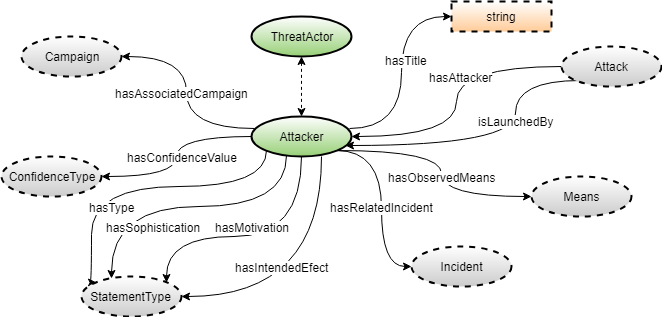
\includegraphics[scale=0.7]{diagramy/Attacker}}
\label{fig:ucoIdentita}
\caption{UCO ontológia -- časť Identita}
\end{figure}


\textbf{Útok} máme reprezentovaný triedou \textit{Attack}, ktorá má viaceré pravidlá na splnenie. Musí mať minimálne jeden význam (\textit{Means}) a minimálne jeden následok (\textit{Consequence}) útoku. Samotný význam je ekvivaletný s triedou TTP, ktorá popisuje samotný útok pomocou informácií o vzoroch útoku, využívaní slabín systémov alebo známych malwaroch. Nakoľko vďaka jazyku OWL vieme definovať napríklad inverzné vlastnosti, je žiadúce, aby sa táto vlastnosť využívala. Pre vlastnoť \textit{hasAttacker} to žiaľ nie je zadefinované a určite by to bolo vhodné zadefinovať.\\
%
\assignment{MH: $\uparrow$ Tu zasa strasne skaces, viac vysvetluj... Kde sa vzalo TTP? Tiez pises, ze \emph{hasAttacker} nie je definovane, ale v tabulke to je...\\
MR: tym som povedal ze nie je zadefinovana ziadna inverzna vlastnost k vlastnosti \textit{hasAttacker}\\
MH: Ano, ale je to tu take vlepene, citatel nechape, preco prave tu uvadzas takuto poznmaku, navyse, asi sa to tyka aj inych vlasnosti, ku ktorym by sa dala dodefinovat inverzna (?) A dalsia vec, nadvazujeme niekde na to? Navrhujeme vylepsenia tohto druhu?}
%
\begin{table}[hbt!]
\centering
\begin{tabular}{ |p{5cm}||p{3cm}|p{3cm}|  }
 \hline
 \multicolumn{3}{|c|}{Útok -- Attack} \\
 \hline
 Vlastnosť & Doména & Rozsah\\
 \hline
 hasAttacker & Attack & Attacker\\
 hasConfidenceValue & Attack & ConfidenceType\\
 hasIndicator & Attack & Indicator\\
 hasMeans & Attack & Means\\
 hasObservable & Attack & Observable\\
 hasRequestedCOA & Attack & CourseofAction\\
 hasSource & Attack & Source\\
 hasTakenCOA & Attack & CourseofAction\\
 isLaunchedBy & Attack & Attacker\\
 \hline
\end{tabular}
\caption{Tabuľka vlastností popisujúcej časť \textbf{Útok} z CTI modelu.}
\label{tab:template}
\end{table}
\begin{figure}[!hb]
\makebox[\textwidth]{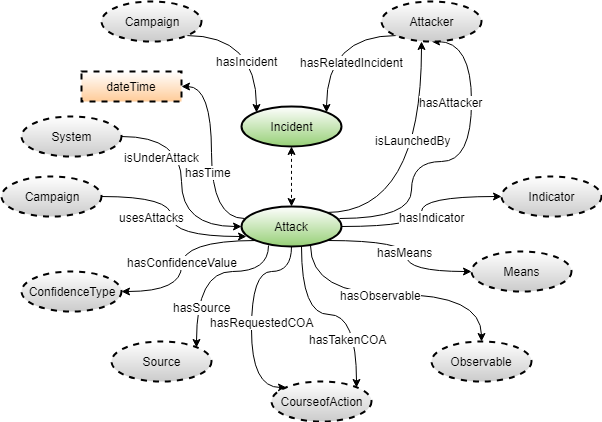
\includegraphics[scale=0.7]{diagramy/Attack}}
\label{fig:ucoUtok}
\caption{UCO ontológia -- časť Útok}
\end{figure}

\textbf{Kampaň} je zahrnutá v triede \textit{Campaign}, ktorá môže existovať iba v prípade, že už bola použitá v nejakom útoku. Každá kampaň môže taktiež mať nejakú ďalšiu kampaň, ktoré medzi sebou súvisia, kde táto vlastnosť je obojsmerná. Taktiež má vlastnosť hasCampaign, ktorej doménou je trieda \textit{Indicator}. Táto trieda pochádza z ontológie CAPEC, ktorá obsahuje známe vzory útokov.
\assignment{MH: $\updownarrow$ Tu (ale aj inde) je taky problem, ze v tabulke je mnozstvo vlastnosti triedy Attack, ci Campaign, ale v texte vysvetlujes len niektore. Nemusis vsetky vymenovavat, ale mozno by sa dalo aspon zhrnut, zgurpit ich... Nieco ako: Ostatne vlasntosti triedy Attak definuju/umoznuju priradit/... ...}
\begin{table}[hbt!]
\centering
\begin{tabular}{ |p{5cm}||p{3cm}|p{3cm}|  }
 \hline
 \multicolumn{3}{|c|}{Kampaň -- Campaign} \\
 \hline
 Vlastnosť & Doména & Rozsah\\
 \hline
 hasAssociatedCampaign & Campaign & Campaign\\
 hasCampaign & Indicator & Campaign\\
 hasIndicator & Campaign & Indicator\\
 hasIncident & Campaign & Incident\\
 hasMenas & Campaign & Means\\
 hasStatus & Campaign & \\
 isLaunchedBy & Campaign & Attacker\\
 usesAttacks & Campaign & Attack\\
 \hline
\end{tabular}
\caption{Tabuľka vlastností popisujúcej časť \textbf{Kampaň} z CTI modelu.}
\label{tab:template}
\end{table}


\textbf{Slabiny} sú zahrnuté v triede \textit{Vulnerability}, ktorá nie je namapovaná na žiadnnu existujúcu ontológiu, avšak dáta už existujú v rámci databázy CVE, ktorá predstavuje dáta o softvérových a hardvérvých chybách. Tieto slabiny sú naviazané na objekty typu \textit{Product} vlastnosťou \textit{affectsProduct}, ktoré môžu byť buď hardvérové alebo softvérové a každá slabina ovplyvňuje niektorý produkt. Taktiež je v nej zaznamený čas objavenia (\textit{discoveryTime}), spôsob narušenia alebo preniknutia do systému (\textit{hasAccessVector}), zložitosť preniknutia do systému (\textit{hasAccessComplexity}), rôzne typy dopadov alebo skóre úspešnosti (\textit{score}). Môže niesť aj informáciu o zdroji slabiny. Taktiež definuje objekty, ktoré je potrebné pozorovať, ktoré sú typu \textit{Observable}. Táto trieda zatiaľ nie je namapovaná na žiadnu existujúcu, ale vieme že existuje ontológia CyBox, ktorá tieto dáta uchováva. 
\begin{table}[hbt!]
\centering
\begin{tabular}{ |p{5cm}||p{3cm}|p{3cm}|  }
 \hline
 \multicolumn{3}{|c|}{Slabina -- Vulnerability} \\
 \hline
 Vlastnosť & Doména & Rozsah\\
 \hline
 affectsProduct & Vulnerability & Product\\
 discoveryTime & Vulnerability & xsd:dateTime\\
 exploitsVulnerability & Means & Vulnerability\\
 hasAccessComplexity & Vulnerability & xsd:string\\
 hasAccessVector & Vulnerability & xsd:string\\
 hasConsequences & Vulnerability & Consequence\\
 hasCVE\_{}ID & Vulnerability & CVE\\
 hasMeans & Vulnerability & Means\\
 hasObservable & Vulnerability & Observable\\
 publishedDateTime & Vulnerability & xsd:dateTime\\
 score & Vulnerability & xsd:float\\
 \hline
\end{tabular}
\caption{Tabuľka vlastností popisujúcej časť \textbf{Slabina} z CTI modelu.}
\label{tab:template}
\end{table}
\begin{figure}[!hb]
\makebox[\textwidth]{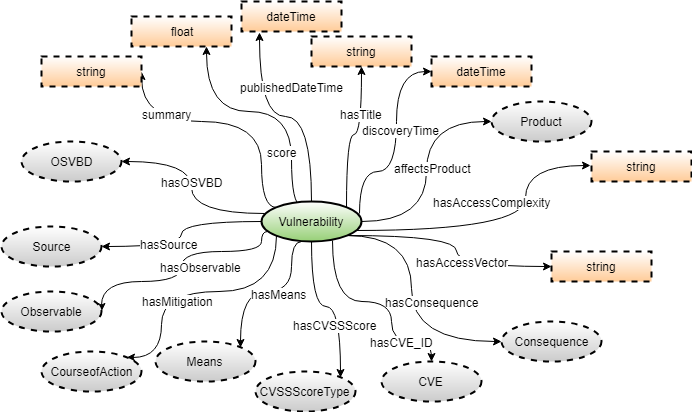
\includegraphics[scale=0.7]{diagramy/Vulnerability}}
\label{fig:ucoSlabiny}
\caption{UCO ontológia -- časť Slabiny}
\minor{MH: CVE -> CWE?}
\end{figure}

Taktiež existuje trieda \textit{CWE}, ktorá je prepojená s triedou \textit{Weakness} z už existujúcej CWE databázy. Taktiež ako trieda \textit{Vulnerability}, popisuje slabiny z CTI modelu. Trieda \textit{CWE} popisuje známe typy slabostí hardvérov a softvérov. Obsahuje informáciu o čase zistenia (\textit{timeOfIntroduction}) a stručný popis (\textit{description}). Zvyšné vlastnosti nemajú definované rozsahy, čo je výrazným nedostatkom a je potrebné tieto vlastnosti dodefinovať.
\assignment{MH: $\uparrow$ V tabulke 5.4 vsak ale vsetky vlastnosti maju aj rozsah, o ktore zvysne teda ide?}
%\textbf{TODO} - zakomponovat mozno zmenu a prepojit to s touto existujúcou databázou. \url{https://cwe.mitre.org/index.html}
\begin{table}[hbt!]
\centering
\begin{tabular}{ |p{5cm}||p{3cm}|p{3cm}|  }
 \hline
 \multicolumn{3}{|c|}{Slabina -- CWE} \\
 \hline
 Vlastnosť & Doména & Rozsah\\
 \hline
 timeOfIntroduction & CWE & xsd:dateTime\\
 discoveryTime & CWE & xsd:dateTime\\
 commonConsequences & CWE & Consequences\\
 \hline
\end{tabular}
\caption{Tabuľka vlastností popisujúcej časť \textbf{Slabina} z CTI modelu.}
\label{tab:template}
\end{table}

\textbf{Indikátory} sú reprezentované triedou \textit{Indicator}. Táto trieda je namapovaná na už existujúcu triedu z ontológie CAPEC. Indikátory spadajú pod kampane (\textit{hasCampaign}) a majú určitý dopad (\textit{hasImpact}). Každý indikátor má aj význam (\textit{hasMeans}) a objekty na pozorovanie z triedy \textit{Observable} (\textit{hasObservable}). Každý indikátor môže mať nejaký iný indikátor, ktorý s ním súvisí (\textit{hasRelatedIndicator}). Obsahuje aj navrhovaný postup reprezentovaný triedou \textit{CourseOfAction} (\textit{hasSuggestedCOA}).
\begin{table}[hbt!]
\centering
\begin{tabular}{ |p{5cm}||p{3cm}|p{3cm}|  }
 \hline
 \multicolumn{3}{|c|}{Indikátory -- Indicator} \\
 \hline
 Vlastnosť & Doména & Rozsah\\
 \hline
 hasCampaign & Indicator & Campaign\\
 hasConfidenceValue & Indicator & ConfidenceType\\
 hasImpact & Indicator & StatementType\\
 hasIndicator & CWE & Indicator\\
 hasKillChainPhase & Indicator & KillChainPhase\\
 hasMeans & Indicator & Means\\
 \hline
\end{tabular}
\caption{Tabuľka vlastností popisujúcej časť \textbf{Indikátor} z CTI modelu.}
\label{tab:template}
\end{table}


\textbf{Nástroje}
TODO -- chcem sa pobavit s panom baloghon co by radil medzi ne z uco ontologie, nakolko sa nevidim tolko do tejto domeny aby som vedel povedat ktora do toho spada.


\chapter{Návrh ontológií}
V predchádzajúcej časti sme si podrobnejšie predstavili vybranú časť UCO ontológie. Ukázali sme si, aké časti z CTI modelu spĺňa a aké dáta jednotlivé okruhy reprezentujú. Touto podrobnejšou anlýzou sme zistili, ktoré dáta ešte nepokrývajú alebo sa nemapujú na už existujúce dáta. 


V tejto kapitole si ukážeme databázy CVE a OVAL, ktoré predstavujú z CTI modelu časť Zraniteľnosť. Predstavíme si nami vytvorené ontológie, ich mapovania a vlastnosti jednotlivých objektov.
\section{CVE}
Common Vulnerabilities and Exposures(CVE)\citep{cve} je databáza všetkých chýb zabezpečenia v oblasti kybernetickej bezpečnosti. Jej úlohou je identifikovať, definovať a katagolizovať tieto chyby, ďalej zraniteľnosti. Každá zraniteľnosť má vlastný záznam, ktorý prechádza fázami v databáze. Zraniteľnosť je najprv objavená, potom pridelená a nakoniec zverejnená. Zverejňovať tieto zraniteľnosti môžu iba tí, ktorí majú partnerstvo s programom CVE. Tieto organizácie dostanú pridelenú množinu CVE záznamov pre daný rok, ktorú môžu postupne napĺňať rôznymi zraniteľnosťami, ktoré objavia. CVE záznamy sú následne používané pri komunikácii a riešení rôznych bezpečnostných hrozieb, aby sa zabezpečilo rovnaké chápanie problému, ktoré bolo konzistentne definované v CVE.  


Tieto záznamy majú svoje identifikátory, ktoré sa skladajú z prefixu \textit{CVE}, následne obsahujú rok objavenia a nakoniec unikátny identifikátor v rámci tejto trojkombinácie oddelenej pomlčkami. Napríklad identifikátor \textit{CVE-2020-0035} predstavuje  zraniteľnosť z roku 2020 v databáze CVE s identifikátorom v danom roku 0035. Podľa množstva záznamov za daný rok, sa odvíja počet cifier na definovanie identifikátora zraniteľnosti. Napríklad v roku 1999, kedy sa začala databáza CVE napĺňať, dosahoval počet zraniteľností ročne 1 600 záznamov, kdežto za rok 2020 to bolo 36 282 záznamov.


\begin{figure}[!hb]
\makebox[\textwidth]{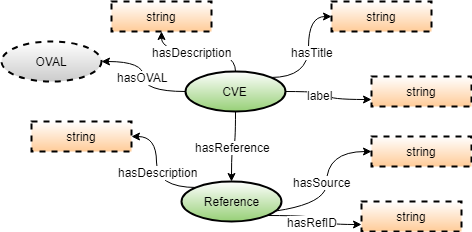
\includegraphics[scale=0.7]{images/cve-ontology}}
\label{fig:cveOnto}
\caption{CVE ontológia}
\end{figure}


Každý jeden záznam má taktiež popis, ktorý musí obsahovať dostatok informácií o tom, na ktoré systémy má daná zranitenosť vplyv, pokiaľ sa vzťahuje aj na konkrétnu verziu, aj táto verzia by mala byť uvedená. Musí obsahovať aj infomácie o type zraniteľnosti, jej príčinu a dopad. Daný popis musí byť napísaný v angličtine.


Záznamy majú aj zoznam referencií, ktoré sú používané ako externé zdroje k zraniteľnosti. Sú to externé odkazy s infomáciou o zdrojovom systéme. Tieto odkazy musia používať iba protokoly \textit{http}, \textit{ftp}, \textit{https}, alebo \textit{ftps}.


Na základe týchto informácií sme vytvorili ontológiu, ktorá obsahuje základné informácie zraniteľnosti, podľa požiadaviek štandardu. Ako definíciu zraniteľnosti, používame jej URI, ktorá poskytuje prepoužitie a odkazovanie sa na ňu. Táto zraniteľnosť má taktiež svoj názov, ktorý reprezentujeme ako CVE identifikátor. Každá zraniteľnosť má svoj popis a zoznam referencií. Ako rozšírenie sme použili vlastnosť \textit{hasRefId}, ktorá definuje unikátny identifikátor, v referencovanom systéme. Tento parameter nie je povinný.




\section{OVAL}
Open Vulnerability and Assessment Language(OVAL)\citep{oval} je štandard, ktorý umožňuje popísanie zraniteľností jednotlivých produktov (softvérov). Tieto informácie sú písané vo formáte XML. Obsahuje tri hlavné kroky posudzovania.


Prvým krokom sú základné informácie o systémoch, ako napríklad o aký operačný systém sa jedná, ktoré jeho verzie ohrozuje a aké konkrétne produkty sú ohrozené, pokiaľ je splnená konfigurácia rôznych systémov. Taktiež obsahuje rôzne odkazy na ďaľšie informácie o jednotlivých zraniteľnostiach. 


Druhé posudzovanie analyzuje systém podľa špecifikovaného nastavenia a zisťuje, či je daný systém ohrozený alebo nie. 


Posledný krok tvorí správu o výsledku tejto analýzy. Na výstupe je informácia o aktuálnom konfiguračnom nastavení systému.


Pre našu ontológiu nie je potrebné reprezentovať všetky znalosti o OVAL-e. Vybrali sme si konkrétne časti, ktoré je potrebné publikovať v našich spravodajských dátach. 


V ontológii reprezentujeme všeobecné informácie popisujúce a definujúce OVAL záznamy, ich vzťahy s jednotlivými operačnými systémami, ich verziami a produktami. Nakoľko vieme že jednotlivé operačné systémy majú rôzne verzie, vieme aj tieto dáta napävno spájať. Zahŕňame aj informácie o externých zdrojoch pre záznamy. Túto vlastnosť prepoužívame z vyššie definovanej časti \textbf{6.1 CVE}. Oproti CVE ale tieto dáta nemajú popis. Túto vlastnosť ale ponecháme, kôli možnému rozšíreniu. OVAL záznami sa taktiež referencujú na rôzne CVE záznamy, ktoré podrobnejšie popisujú. V našej ontológii takýto typ referencie budeme popisovať špecifickou vlastnosťou.


Taktiež predpripravíme ontológiu na reprezentovanie kritérií, ktoré predstavujú logické testy. Tieto testy majú v sebe aj výrokovú logiku reprezentovanú pomocou logických operátorov AND a OR, kde je možné definovať viacúrovňové logické výrazy. Jednotlivé kritéria majú stručný popis a obšírnejší popis, kde sú definované jednotlivými testami alebo ďalšími OVAL záznamami.


\begin{figure}[!hb]
\makebox[\textwidth]{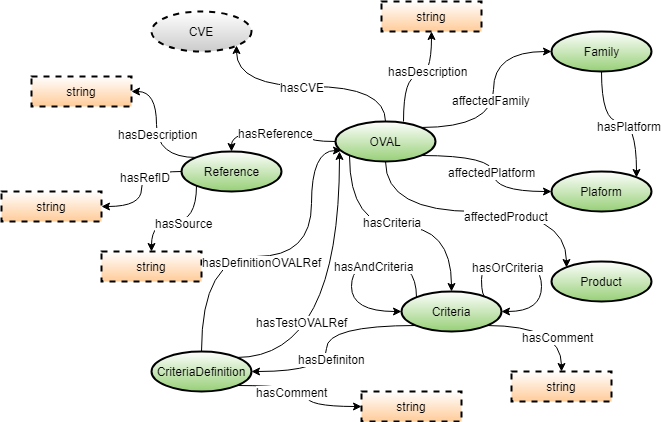
\includegraphics[scale=0.7]{images/oval-ontology}}
\label{fig:ovalOnto}
\caption{OVAL ontológia}
\end{figure}


Každý OVAL objekt je reprezentovaný pomocou URN \textit{oval:org.cisecurity:\{def\}:127} kde \textit{\{def\}} musí byť z nasledujúcich možností:
\begin{itemize}
\item \textbf{def} -- jedná sa o záznam definujúci zraniteľnosť
\item \textbf{tst} -- záznam, ktorý definuje test
\item \textbf{var} -- záznam definujúci množinu verzií platformy alebo produktu
\item \textbf{obj} -- príkaz, ktorý je potrebný spustiť v konzole
\item \textbf{ste} -- objekt, popisujúci výstup z konzoly s definovanou operáciou na kontrolu ako je regulárny výraz, porovnanie alebo výber z množiny verzií
\end{itemize}
Samotný záznam sa skladá z:
\begin{itemize}
\item \textit{hasTitle} -- názov záznamu
\item \textit{hasDescription} -- popis záznamu
\item \textit{affectedFamily} -- operačný systém, ktorý ovplyvňuje
\item \textit{affectedPlatform} -- akú platformu operačného systému ovplyvňuje
\item \textit{affectedProduct} -- ktorý produkt ovplyvňuje
\item \textit{hasReference} -- odkaz na externý zdroj informácií súvisiaci so záznamom
\item \textit{hasCriteria} -- zoznam logických testov potrebených na zistenie či daný záznam ovplyvňuje systém
\item \textit{hasCVE} -- CVE objekt, ktorý popisuje daný OVAL záznam
\end{itemize}
Kritériá popisujúce test majú nasledujúce vlastnosti:
\begin{itemize}
\item hasAndCriteria -- logické pravidlo spojené s rodičom AND operátorom
\item hasOrCriteria -- logické pravidlo spojené s rodičom OR operátorom
\item hasDefinition -- definícia kritéria
\item hasComment -- popis kritéria alebo definície kritéria
\item hasTest -- definícia vykonania a kontroly výstupu z testu
\end{itemize}



\chapter{Implementácia a testovanie}
V kapitole Návrh ontológií sme si predstavili nami vytvorené ontológie z už existujúcich databáz CVE a OVAL.


V tejto kapitole si ukážeme ako sme na tieto ontológie namapovali už existujúce dáta, ako sme tieto dáta migrovali a ako ich reprezentujeme na webe. Taktiež si ukážeme rôzne príklady použitia a analýzy nad importovanými dátami.
\section{Dáta}
Dáta, ktoré sme spracovávali pochádzajú z verejne dostupného zdroja štandardov OVAL a CVE. Tieto dáta mali pôvodne štruktúru XML, ktorá ale nebola písaná OWL syntaxov. Tieto dáta sme spracovali pomocou programovacieho jazyka Python. Jednotlivé triedy v nami navrhnutých ontológiách sme si implementovali a následne sme spracovali dané dátové súbory pomocou knižnice \textit{xml}. Po sparsovaní dát sme tieto dáta definovali pomocou tripletov a následne ich zapísali pomocou knižnice \textit{rdflib} do súboru vo formáte \textit{turtle}. 


Tento formát sme vybrali najmä kôli menšiemu objemu dát, nakoľko bolo potrebných viac optimalizácií pre generovanie. Ale aj po tejto optimalizácii sme nevedeli spracovať niektoré skupiny záznamov, preto sme sa  rozhodli ich rozdeliť. CVE dáta sme spracovali tak, že sme ich rozdelili podľa rokov vytvorenia. OVAL dáta sme rozdelili podľa operačného systému, ktorého sa týkajú. Po zapísaní časti dát, sme túto časť premazali z pamäte a prešli sme na ďalšiu časť.


Nakoniec sme tieto migrované dáta nahrali na webovú službu github, ktorá poskytuje možnosť nahrávať zdrojové súbory do repozitára.


\section{Testovanie}
V predchádzajúcich častiach sme si popísali ako sme dáta migrovali a mapovali na nami vytvorenú ontológiu. Taktiež sme si popísali webovú stránku, ktorú sme vytvárali v spolupráci so študentami z FEI STU, ktorá slúži na zobrazovanie našich dát.


V tejto kapitole sa budeme venovať testovaniu našej vygenerovanej ontológie a dopytovanie sa nad nami importovanými dátami. Ukážeme si rôzne testy použiteľnosti a ukážky SPARQL dopytov.


\subsection{Príklady použitia}
Všetky nasledujúce príklady použitia boli overené na lokálne nainštalovanom triple store, do ktorého sme si naimportovali všetky migrované dáta. Každý jeden SPARQL dopyt sme sputili a na základe jeho výsledkov sme vyhodnocovali jednotlivé prípady použitia.
\subsection*{Príklad 1}
\label{sec:priklad1}
\subsubsection*{Názov}
CVE podľa platformy

\subsubsection*{Zadanie}
Podľa zadanej platformy, nájdi v databáze všetky CVE objekty, ktoré súvisia s danou platformou. Na výstupe vráť ich URI definíciu s názvom CVE záznamu.

\subsubsection*{Dopyt}
\begin{small}
\begin{verbatim}
PREFIX main: <http://www.semanticweb.org/rycht/ontologies
  /cyber_security_ontology#>
PREFIX platform: <http://www.semanticweb.org/rycht/ontologies
  /cyber_security_ontology/platform#>
PREFIX cve: <https://cve.mitre.org/about/terminology.html#>
PREFIX oval:<https://oval.mitre.org/language/version5.11/OVAL>

SELECT ?cve ?title
WHERE {
  ?cve a cve:CVE.
  ?cve main:hasTitle ?title.
  ?oval a oval:.
  ?oval main:hasCVE ?cve.
  ?oval main:affectedPlatform platform:Some_platform
}
\end{verbatim}
\end{small}


\subsubsection*{Výstup}
Nad výstupom tohoto dopytu sme spravili analýzu, kde sme zistili, že najčastejšie vyskytujúca sa platforma mala priradených skoro 10 000 CVE záznamov z aktuálnych 204 144.


\subsection*{Príklad 2}
\label{sec:priklad2}
\subsubsection*{Názov}
OVAL záznamy, ktoré ovplyvňujú iba platformu.

\subsubsection*{Zadanie}
Vráť mi všetky OVAL záznamy, ktoré ovplyvňujú všeobecne platformu a žiaden konkrétny produkt pre danú platformu. Na výstupe mi pošli ich URI OVAL záznamu, názov, URI a názov operačnénho systému a URI a názov platformy.

\subsubsection*{Dopyt}
\begin{small}
\begin{verbatim}
PREFIX main: <http://www.semanticweb.org/rycht/ontologies
  /cyber_security_ontology#>
PREFIX cve: <https://cve.mitre.org/about/terminology.html#>
PREFIX oval:<https://oval.mitre.org/language/version5.11/OVAL>
PREFIX rdfs: <http://www.w3.org/2000/01/rdf-schema#>

SELECT ?oval ?title ?family ?familyName ?platform ?platformName
WHERE {
  ?oval a oval:.
  ?oval main:hasTitle ?title.
  ?oval main:affectedFamily ?family.
  ?family rdfs:label ?familyName.
  ?oval main:affectedPlatform ?platform.
  ?platform rdfs:label ?platformName.
  NOT EXISTS {
    ?oval main:affectedProduct ?product.
  }
}
\end{verbatim}
\end{small}

\subsubsection*{Výstup}
Záznamov, ktoré spĺňajú dané zadanie sme identifikovali z takmer 20 000 oval záznamoch 9 065. Tým sme získali určitú predstavu o počte OVAL záznamoch, ktoré všeobecne ovplyvňujú iba plaformy operačných systémov.


\subsection*{Príklad 3}
\label{sec:priklad3}
\subsubsection*{Názov}
Frekvenčná tabuľka CVE záznamov.

\subsubsection*{Zadanie}
Získaj všetky CVE záznamy, zoradené podľa toho, ako často sú využívané ako referencia v OVAL záznamoch. Zoraď ich podľa využívanosti od najväčšej a na výstup vráť URI a názov CVE záznamu s počtom OVAL definícií, v ktorých sú použité.

\subsubsection*{Dopyt}
\begin{small}
\begin{verbatim}
PREFIX main: <http://www.semanticweb.org/rycht/ontologies
  /cyber_security_ontology#>
PREFIX platform: <http://www.semanticweb.org/rycht/ontologies
  /cyber_security_ontology/platform#>
PREFIX cve: <https://cve.mitre.org/about/terminology.html#>
PREFIX oval:<https://oval.mitre.org/language/version5.11/OVAL>

SELECT ?cve ?title (COUNT(?oval) as ?count)
WHERE {
  ?cve a cve:CVE.
  ?cve main:hasTitle ?title.
  ?oval a oval:.
  ?oval main:hasCVE ?cve.
} 
GROUP BY ?cve ?title
ORDER BY DESC(?count)
\end{verbatim}
\end{small}


\subsubsection*{Výstup}
Najviac používaný CVE záznam v OVAL záznamoch bol odkazovaný 12 krát. Zvyšné záznamy boli vždy odkazované aspoň 1 krát, teda sme zistili, že každý CVE záznam je podrobnejšie popísaný v OVAL záznamoch. Neexistuje záznam, ktorbý by nebol spracovaný v OVAL databáze.


\subsection*{Príklad 4}
\label{sec:priklad4}
\subsubsection*{Názov}
Cve záznamy ovplyvňujúce viac operačných systémov.


\subsubsection*{Zadanie}
Nájdi také CVE záznamy, ktoré ovplyvňujú rovnaký produkt na rôznych operačných systémoch. Na výstup vráť URI a názov CVE záznamu, produkt ktorý ovplyvňuje a URI operačných systémov.


\subsubsection*{Dopyt}
\begin{small}
\begin{verbatim}
PREFIX main: <http://www.semanticweb.org/rycht/ontologies
  /cyber_security_ontology#>
PREFIX platform: <http://www.semanticweb.org/rycht/ontologies
  /cyber_security_ontology/platform#>
PREFIX cve: <https://cve.mitre.org/about/terminology.html#>
PREFIX oval:<https://oval.mitre.org/language/version5.11/OVAL>

SELECT ?cve ?title ?product ?family1 ?family2
WHERE {
  ?cve a cve:CVE.
  ?cve main:hasTitle ?title.
  ?oval1 a oval:.
  ?oval1 main:hasCVE ?cve.
  ?oval1 main:affectedProduct ?product.
  ?oval1 main:affectedFamily ?family1.
  ?oval2 a oval:.
  ?oval2 main:hasCVE ?cve.
  ?oval2 main:affectedProduct ?product.
  ?oval2 main:affectedFamily ?family2.
  FILTER (?family1 != ?family2).
} 
\end{verbatim}
\end{small}


\subsubsection*{Výstup}
Počet CVE záznamov, ktoré ovplyvňujú viac ako jeden operačný systém je z 204 144 CVE záznamov 146.



\section{Internetová stránka}
V spolupráci so študentami môjho konzultanta, sme vytvorili internetovú stránku, založenú na našej ontológii a našich vygenerovaných dátach. Táto stránka bude skúžiť na zobrazenie CVE a OVAL dát, kde bude možné tieto dáta prezerať a vyhľadávať. Pomocou SPARQL dopytov sa vyhľadávajú jednotlivé dáta a ich konkrétne informácie.


Takiež sa v nej budú dať prezerať dáta o jednotlivých operačných systémoch, ich platformách a produktoch. Na týchto stránkach budú informácie o jednotlivých OVAL a CVE záznamoch, ktoré sa týkajú daného predmetu.


Základná stránka pre každý OVAL a CVE objekt bude zobrazovať všetky dáta, ktoré má v databáze definované na prvej úrovni t.j. dáta, kde daný objekt figuruje ako predmet v trojici. 



\chapter{Záver}

V tejto práci sme vykonali analýzu rôznych existujúcich ontologických riešení v
oblasti publikovania spravodajských dát o bezpečnostných hrozbách. Nakoniec sme
sa zamerali na ontologické riešenie UCO, ktoré sme najprv vyhodnotili vzhľadom
na CTI model, ktorý definuje oblasti, ktoré je potrebné zaznamenávať. Tieto oblasti aj bližšie definuje a popisuje. Následne sme zhodnotili, aké časti nie sú dostatočne zapracované
v tejto ontológii a túto časť sme rozšírili o ontológiu, ako aj o dáta z
verejných databázových riešení OVAL a CVE, ktoré popisujú zraniteľnosti
operačných systémov, ich platforiem a produktov.

\assignment{MH $\uparrow$ Ten CTI model trochu uved vysvetli, ked ho prvy raz spominas v zavere,
pre pripad, ze niekto zacne citat od zaveru (komisia)\\
MR: rozpisany\\
MH: Myslel som rozpisat skratku, ale to vysvetlenie je tiez fajn...}

Týmto rozšírením sme získali úplnejšiu ontológiu, ktorá vo väčšej miere pokrýva CTI model, ktorý bol naším referenčným modelom.


Dáta v jednotlivých databázových riešeniach sme zanalyzovali, na základe týchto dát sme vytvorili ontologické riešenie, ktoré pokrývalo všetky dáta relevantné pre publikovanie a tieto vybraté dáta sme zmapovali na naše ontologické riešenia. Nad týmito dátami sme následne vytvorili rôzne analýzy a prípady použitia na popis, čo sa v nami navrhnutých ontológiách dá zistiť.


\section*{Prínos}
Pomocou ontologického riešenia, časti z domény kybernetickej bezpečnosti, sa nám podarilo vyjadriť tieto dáta vo jednotnej forme, prepojiť naše riešenie s už existujúcim štandardom repreznetovania znalostí v doméne kybernetickej bezpečnosti, ako aj jej rozšírenie o časť zraniteľnosti a ich podrobný popis. Podarilo sa nám premapovať existujúce OVAL a CVE dáta na naše ontologické riešenie a poprepájať tieto dáta medzi sebou.

Vďaka tomu vieme tieto dáta reprezentovať a publikovať na webe, v sieti prepojených dát vo forme, ktorá je prepoužiteľná a
strojovo čitateľná. Hocikto sa môže na naše dáta odkazovať, opätovne ich využiť alebo rozšíriť. 

\assignment{MH: $\uparrow$ Az teraz som si vsimol, ze mas jednopismenkove slova na konci riadku. To nie je v slovencine OK, pouzi nedelitelnu medzeru (v LaTeXu znak tilda). Treba fixnut vsade v celej praci}

Naša práca taktiež dokáže pomôcť pri prevencii a ochrane pred
kybernetickými hrozbami. Vďaka dátam, ktoré sme importovali do našej ontológie, vieme vyhodnocovať jednotlivé zraniteľnosti pre operačné systémy, platformi a produkty a taktiež vieme povedať, aké všetky produkty ovplyvňuje CVE alebo OVAL záznam. Vieme identifikovať záznamy, ktoré sa týkajú iba platforiem všeobecne, alebo také, ktoré sa využívajú najčastejšie.


Táto práca je zároveň súčasťou projektu ORBIS (APVV-19-0220) v rámci ktorého vzniká dátové úložisko o bezpečnostných hrozbách a internetová stránka na ich prezeranie. Tento projekt sa stavia aj na základe nami vytvorenej ontológie a využije ju ako základ, ktorý sa postupne bude rozrastať o ďalšie ontologické riešenia.

\assignment{MH: $\uparrow$ Najma, co si nenapisal, ze Tvoju ontologiu pouzie na
repreznetaciu dat v tom ulozisku. Tiez, toto je praca, ktora na teba nadvazuje,
tak by som to dal do Buduceho pokracovania, aj ked uz sa siastocne deje...}

\section*{Budúce pokračovanie}
\overview{MH: Kde vidime priestor, ze co by s tym niekto mohol robit, dalsie mozne vylepsenia}
OVAL databáza poskytuje aj popis jednotlivých sád testov, podmocou ktorých sa vyhodnocuje, či je systém ohrozený alebo nie. Na spojenie týchto dát s našou ontológiou by bolo potrebné hlbšie preskúmať logickú sémantiku ich jazyka. V našej ontológii už sú predpripravené mapovania na tieto testy.


Možným pokračovaním je aj možnosť rozšíriť ontológiu UCO o ďalšie mapovania na už existujúce databázy, kde môžu už mať ontologické riešenie alebo takéto ontologické riešenie bude potrebné vytvoriť. Následne extrahovať relevantné dáta z takejto databázy a pokúsiť sa namapovať ich na nami naimportované dáta. Takýmito dátami môžu byť napríklad dáta, ktoré poskytuje databáza ATT\&{}CK\citep{attck}, kde je zahrnutá znalosť o taktikách a technikách útoku.

\assignment{MH: $\uparrow$ Zahadne \uv{dalsie databazy}, uved aspon nejaky priklad, ak vies\\
MR: dodana ATT\&{}CK\citep{attck}}



\assignment{MH: $\uparrow$ Opat, toto je velmi velmi vagne, a moze to budit dojem, ze ani nam samym to nie je uplne jasne.\\
MR: ina formulacia zaveru\\
MH: Tato posledna veta je stale rovnako vagna, ake dalsie analyzy?\\
MR: tie analyzy sa tazko popisuju, kedze nikdy nevies co ti z analyzy moze vypadnut, nechal som to radsej tak a vymazal to}
\assignment{MH: $\uparrow$ No a co mi tu uplne chyba, je spomenut sirsi kontext projektu ORBIS, vdaka ktoremu na zaklade Tvojej ontologie vznikde semaniticky repozitar, do ktoreho skutocne budu tie data naimportovane a zverejnene.\\
MH (new): Ty si sa ale ani nepokusil napisat nieco o tom ako na tvoju pravu nadvazuju studenti z FEI. Ked to napises, tak sa tam odvolaj na to, ze \uv{Tato praca (ako Tvoja) je sucastou sirsieho
projektu ORBIS (APVV-19-0220), v ramci ktoreho vznika aj datove ulozisko...}, ktore stavia na Tvojej ontologu, a vyuzije ju tak a tak, a jeho cielom a prinosom bude...\\
MR: zapracovana cast ORBIS do prinosu prace}

\nocite{*}
\bibliographystyle{alpha}
\bibliography{references}

\listoffigures

\end{document}
